\documentclass[11pt]{article}\usepackage[]{graphicx}\usepackage[]{color}
%% maxwidth is the original width if it is less than linewidth
%% otherwise use linewidth (to make sure the graphics do not exceed the margin)
\makeatletter
\def\maxwidth{ %
  \ifdim\Gin@nat@width>\linewidth
    \linewidth
  \else
    \Gin@nat@width
  \fi
}
\makeatother

\definecolor{fgcolor}{rgb}{0.345, 0.345, 0.345}
\newcommand{\hlnum}[1]{\textcolor[rgb]{0.686,0.059,0.569}{#1}}%
\newcommand{\hlstr}[1]{\textcolor[rgb]{0.192,0.494,0.8}{#1}}%
\newcommand{\hlcom}[1]{\textcolor[rgb]{0.678,0.584,0.686}{\textit{#1}}}%
\newcommand{\hlopt}[1]{\textcolor[rgb]{0,0,0}{#1}}%
\newcommand{\hlstd}[1]{\textcolor[rgb]{0.345,0.345,0.345}{#1}}%
\newcommand{\hlkwa}[1]{\textcolor[rgb]{0.161,0.373,0.58}{\textbf{#1}}}%
\newcommand{\hlkwb}[1]{\textcolor[rgb]{0.69,0.353,0.396}{#1}}%
\newcommand{\hlkwc}[1]{\textcolor[rgb]{0.333,0.667,0.333}{#1}}%
\newcommand{\hlkwd}[1]{\textcolor[rgb]{0.737,0.353,0.396}{\textbf{#1}}}%

\usepackage{framed}
\makeatletter
\newenvironment{kframe}{%
 \def\at@end@of@kframe{}%
 \ifinner\ifhmode%
  \def\at@end@of@kframe{\end{minipage}}%
  \begin{minipage}{\columnwidth}%
 \fi\fi%
 \def\FrameCommand##1{\hskip\@totalleftmargin \hskip-\fboxsep
 \colorbox{shadecolor}{##1}\hskip-\fboxsep
     % There is no \\@totalrightmargin, so:
     \hskip-\linewidth \hskip-\@totalleftmargin \hskip\columnwidth}%
 \MakeFramed {\advance\hsize-\width
   \@totalleftmargin\z@ \linewidth\hsize
   \@setminipage}}%
 {\par\unskip\endMakeFramed%
 \at@end@of@kframe}
\makeatother

\definecolor{shadecolor}{rgb}{.97, .97, .97}
\definecolor{messagecolor}{rgb}{0, 0, 0}
\definecolor{warningcolor}{rgb}{1, 0, 1}
\definecolor{errorcolor}{rgb}{1, 0, 0}
\newenvironment{knitrout}{}{} % an empty environment to be redefined in TeX

\usepackage{alltt}

\usepackage{amsmath}
\usepackage{amsfonts}
\usepackage{xfrac}

\usepackage{fullpage}
\usepackage{parskip}
\usepackage{booktabs}
\usepackage{graphicx}
\usepackage{caption}
% \usepackage{subfig}
\usepackage{subcaption}
\newcommand{\subfloat}[2][need a sub-caption]{\subcaptionbox{#1}{#2}}
% \usepackage{subfig}
% \usepackage{movie15}
% \usepackage{animate}

\usepackage[hidelinks]{hyperref}




\newcommand{\bx}{\boldsymbol{x}}
\newcommand{\bu}{\boldsymbol{u}}
\newcommand{\bw}{\boldsymbol{w}}
\newcommand{\bz}{\boldsymbol{z}}
\newcommand{\by}{\boldsymbol{y}}
\newcommand{\bY}{\boldsymbol{Y}}
\newcommand{\br}{\boldsymbol{r}}
\newcommand{\bd}{\boldsymbol{d}}
\newcommand{\bs}{\boldsymbol{s}}
\newcommand{\bh}{\boldsymbol{h}}
\newcommand{\bv}{\boldsymbol{v}}
\newcommand{\bfn}{\boldsymbol{f}}
\newcommand{\bF}{\boldsymbol{F}}
\newcommand{\bg}{\boldsymbol{g}}
\newcommand{\bH}{\boldsymbol{2H}}
\newcommand{\bK}{\boldsymbol{K}}
\newcommand{\bQ}{\boldsymbol{Q}}
\newcommand{\bR}{\boldsymbol{R}}
\newcommand{\bP}{\boldsymbol{P}}
\newcommand{\bS}{\boldsymbol{S}}
\newcommand{\bZero}{\boldsymbol{0}}
\newcommand{\dd}[2]{\frac{\partial {#1}}{\partial {#2}}}

\newcommand{\X}{\mathrm{X}}
\newcommand{\E}{\mathrm{E}}
\newcommand{\V}{\mathrm{V}}


\newcommand{\pr}{\mathbb{P}}
\renewcommand{\Pr}[1]{\pr\left(#1\right)}
\newcommand{\Ex}[1]{\mathbb{E}\left[#1\right]}
\newcommand{\given}{\,|\,}


\newcommand{\km}{_{k-1}}
\newcommand{\kk}{_{k|k}}
\newcommand{\kkm}{_{k|k-1}}
\newcommand{\kmkm}{_{k-1|k-1}}


\title{Modelling Bus Route 090}
\author{}
\date{}
\IfFileExists{upquote.sty}{\usepackage{upquote}}{}
\begin{document}
\maketitle



\section{Initial Historical Data}
\label{sec:historical-data}


A couple of weeks worth of data was collected for the bus route 090 (Westgate to Downtown), 
and a very general Particle Filter model was used to estimate the distance into trip, $\bd$,
of each observation. 
This data is stored in the database \texttt{db/historical\_data.db}.
The following code extracts the raw history, 
and makes a few manipulations to make it easier to work with,
as well as remove some impossibly fast trips.

\begin{knitrout}
\definecolor{shadecolor}{rgb}{0.969, 0.969, 0.969}\color{fgcolor}\begin{kframe}
\begin{alltt}
\hlstd{routeid} \hlkwb{<-} \hlstr{"09001%"}
\hlstd{hist090} \hlkwb{<-} \hlkwd{dbGetQuery}\hlstd{(}\hlkwd{dbConnect}\hlstd{(}\hlkwd{SQLite}\hlstd{(),} \hlstr{"historical-data.db"}\hlstd{),}
                      \hlkwd{sprintf}\hlstd{(}\hlstr{"SELECT * FROM history WHERE route_id LIKE '%s'"}\hlstd{,}
                              \hlstd{routeid))}
\hlstd{hist090}\hlopt{$}\hlstd{time.day} \hlkwb{<-} \hlstd{hist090}\hlopt{$}\hlstd{timestamp} \hlopt{-}
    \hlkwd{as.numeric}\hlstd{(}\hlkwd{format}\hlstd{(}\hlkwd{as.POSIXct}\hlstd{(}\hlkwd{paste}\hlstd{(hist090}\hlopt{$}\hlstd{trip_start_date,}
                                       \hlstr{"00:00:00"}\hlstd{)),}
                      \hlkwc{format} \hlstd{=} \hlstr{"%s"}\hlstd{))}
\hlstd{hist090}\hlopt{$}\hlstd{time.hour} \hlkwb{<-} \hlstd{hist090}\hlopt{$}\hlstd{time.day} \hlopt{/} \hlnum{60} \hlopt{/} \hlnum{60}
\hlstd{hist090}\hlopt{$}\hlstd{dvt} \hlkwb{<-} \hlkwd{as.factor}\hlstd{(}\hlkwd{paste}\hlstd{(hist090}\hlopt{$}\hlstd{trip_start_date,}
                               \hlstd{hist090}\hlopt{$}\hlstd{trip_id,}
                               \hlstd{hist090}\hlopt{$}\hlstd{vehicle_id,}
                               \hlkwc{sep} \hlstd{=} \hlstr{":"}\hlstd{))}
\hlstd{which.keep} \hlkwb{<-}
    \hlkwd{do.call}\hlstd{(c,}
            \hlkwd{invisible}\hlstd{(}\hlkwd{tapply}\hlstd{(}\hlnum{1}\hlopt{:}\hlkwd{nrow}\hlstd{(hist090), hist090}\hlopt{$}\hlstd{dvt,} \hlkwa{function}\hlstd{(}\hlkwc{i}\hlstd{) \{}
                \hlstd{d} \hlkwb{<-} \hlkwd{diff}\hlstd{(}\hlkwd{range}\hlstd{(hist090}\hlopt{$}\hlstd{time.day[i]))}
                \hlstd{dt} \hlkwb{<-} \hlkwd{diff}\hlstd{(hist090}\hlopt{$}\hlstd{time.day[i])}
                \hlstd{dx} \hlkwb{<-} \hlkwd{diff}\hlstd{(hist090}\hlopt{$}\hlstd{distance[i])}
                \hlkwa{if} \hlstd{(}\hlkwd{max}\hlstd{(dx}\hlopt{/}\hlstd{dt)} \hlopt{<} \hlnum{50}\hlstd{)} \hlkwd{return}\hlstd{(i)} \hlkwa{else} \hlkwd{numeric}\hlstd{()}
            \hlstd{\})))}
\hlstd{hist090} \hlkwb{<-} \hlstd{hist090[which.keep, ]}
\hlkwd{with}\hlstd{(hist090,} \hlkwd{plot}\hlstd{(time.hour, distance,} \hlkwc{type} \hlstd{=} \hlstr{"n"}\hlstd{,}
                   \hlkwc{main} \hlstd{=} \hlstr{"History of Route 090"}\hlstd{,} \hlkwc{xlab} \hlstd{=} \hlstr{"Time (h)"}\hlstd{,}
                   \hlkwc{ylab} \hlstd{=} \hlstr{"Distance into Trip (m)"}\hlstd{))}

\hlkwd{invisible}\hlstd{(}\hlkwd{tapply}\hlstd{(}\hlnum{1}\hlopt{:}\hlkwd{nrow}\hlstd{(hist090), hist090}\hlopt{$}\hlstd{dvt,}
                 \hlkwa{function}\hlstd{(}\hlkwc{i}\hlstd{)} \hlkwd{lines}\hlstd{(hist090}\hlopt{$}\hlstd{time.hour[i], hist090}\hlopt{$}\hlstd{distance[i])))}
\end{alltt}
\end{kframe}
\includegraphics[width=\maxwidth]{figure/extract_historical_data-1} 

\end{knitrout}


\section{Predicting a Route}
\label{sec:route_prediction}

From here, we will be using the historical data to project particles ahead to estimate arrival time at future stops.
There will be two parts to each iteration:
\begin{enumerate}
\item predict partical arrival times at future stops,
  
\item predict partical locations at time $t_{k-1} + \delta_k$.
\end{enumerate}
The first will be used to predict arrival time at stops, 
while the second will be used to predict the new location of the bus and produce a new set of particles for the next iteration.


Each bus reports its position at time $t_k$ as $r_k$ (latitude, longitude), 
where the $k$ subscript is the observation number.
The distance into trip at time $t_k$ is defined as $d_k$, 
and is known only as a distribution which is defined by the particles $\bw_k$.
For now, only distance will be used; in future, however, velocity may also be modelled.


The particles are updated using standard Particle Filter theory, 
so that after each new observation is obtained, 
the distribution of the particles represents the posterior distribution of $d_k$ via SIR.


For this example, we will use a single trip:
\begin{knitrout}
\definecolor{shadecolor}{rgb}{0.969, 0.969, 0.969}\color{fgcolor}\begin{kframe}
\begin{alltt}
\hlstd{tripid} \hlkwb{<-} \hlstr{"^3090020609"}
\hlstd{hist} \hlkwb{<-} \hlstd{hist090[}\hlkwd{grepl}\hlstd{(tripid, hist090}\hlopt{$}\hlstd{trip_id), ]}
\hlstd{hist}\hlopt{$}\hlstd{dvt} \hlkwb{<-} \hlkwd{factor}\hlstd{(hist}\hlopt{$}\hlstd{dvt)}
\hlstd{hist}\hlopt{$}\hlstd{time_into_trip} \hlkwb{<-}
    \hlkwd{do.call}\hlstd{(c,} \hlkwd{tapply}\hlstd{(}\hlnum{1}\hlopt{:}\hlkwd{nrow}\hlstd{(hist), hist}\hlopt{$}\hlstd{dvt,}
                      \hlkwa{function}\hlstd{(}\hlkwc{i}\hlstd{) hist}\hlopt{$}\hlstd{time.day[i]} \hlopt{-} \hlkwd{min}\hlstd{(hist}\hlopt{$}\hlstd{time.day[i])))}

\hlstd{test.trip} \hlkwb{<-} \hlstd{hist[hist}\hlopt{$}\hlstd{trip_start_date} \hlopt{==} \hlkwd{tail}\hlstd{(}\hlkwd{unique}\hlstd{(hist}\hlopt{$}\hlstd{trip_start_date),} \hlnum{1}\hlstd{), ]}
\hlstd{hist} \hlkwb{<-} \hlstd{hist[hist}\hlopt{$}\hlstd{trip_start_date} \hlopt{!=} \hlkwd{tail}\hlstd{(}\hlkwd{unique}\hlstd{(hist}\hlopt{$}\hlstd{trip_start_date),} \hlnum{1}\hlstd{), ]}
\hlstd{hist}\hlopt{$}\hlstd{dvt} \hlkwb{<-} \hlkwd{factor}\hlstd{(hist}\hlopt{$}\hlstd{dvt)}

\hlkwd{with}\hlstd{(hist,} \hlkwd{plot}\hlstd{(time_into_trip, distance,} \hlkwc{type} \hlstd{=} \hlstr{"n"}\hlstd{,}
                \hlkwc{main} \hlstd{=} \hlstr{"History of Route 090, 12:15 trip"}\hlstd{,}
                \hlkwc{xlab} \hlstd{=} \hlstr{"Time into Trip (s)"}\hlstd{,}
                \hlkwc{ylab} \hlstd{=} \hlstr{"Distance into Trip (m)"}\hlstd{))}
\hlkwd{invisible}\hlstd{(}\hlkwd{tapply}\hlstd{(}\hlnum{1}\hlopt{:}\hlkwd{nrow}\hlstd{(hist), hist}\hlopt{$}\hlstd{dvt,}
                 \hlkwa{function}\hlstd{(}\hlkwc{i}\hlstd{)} \hlkwd{lines}\hlstd{(hist}\hlopt{$}\hlstd{time_into_trip[i], hist}\hlopt{$}\hlstd{distance[i])))}

\hlstd{stops} \hlkwb{<-} \hlnum{1}\hlopt{:}\hlnum{15} \hlopt{*} \hlnum{2000}
\hlkwd{abline}\hlstd{(}\hlkwc{h} \hlstd{=} \hlkwd{c}\hlstd{(}\hlnum{0}\hlstd{, stops),} \hlkwc{col} \hlstd{=} \hlstr{"#0000ff"}\hlstd{,} \hlkwc{lty} \hlstd{=} \hlnum{3}\hlstd{)}
\end{alltt}
\end{kframe}
\includegraphics[width=\maxwidth]{figure/example_trip-1} 

\end{knitrout}
The first model is going to ignore actual start time, and instead just use variability in travel times.
Also, to simplify, we have made up 15 evently spaced ``stops''.



\subsection{Arrival Times at Future Stops}
\label{sec:future_arrival_times}


The prediction of arrival times is actually fairly straight forward.
We start off with (for simplicity) 50 walkers, $w_0(i), i \in \{1,...,10\}$, 
all starting at zero.

\begin{knitrout}
\definecolor{shadecolor}{rgb}{0.969, 0.969, 0.969}\color{fgcolor}\begin{kframe}
\begin{alltt}
\hlstd{M} \hlkwb{<-} \hlnum{500}
\hlstd{w} \hlkwb{<-} \hlkwd{rep}\hlstd{(}\hlnum{0}\hlstd{, M)}
\end{alltt}
\end{kframe}
\end{knitrout}

From here, we wish to predict $a_1$, arrival time at stop number 1, $s_1$.
To do this, we need to know at what \emph{time} each historical journey arrives at the stop.
This is done by fitting a polynomial spline to each journey, 
and some fancy optimisation techniques to find $a_{1|\boldsymbol{j}}$ 
($\boldsymbol{j}$ represents all of the information associated with historical trip $j$).

\begin{knitrout}
\definecolor{shadecolor}{rgb}{0.969, 0.969, 0.969}\color{fgcolor}\begin{kframe}
\begin{alltt}
\hlstd{history.fn} \hlkwb{<-} \hlkwd{try}\hlstd{(\{}
    \hlkwd{tapply}\hlstd{(}\hlnum{1}\hlopt{:}\hlkwd{nrow}\hlstd{(hist), hist}\hlopt{$}\hlstd{dvt,} \hlkwa{function}\hlstd{(}\hlkwc{i}\hlstd{) \{}
               \hlstd{f}\hlkwb{=}\hlkwd{splinefun}\hlstd{(hist}\hlopt{$}\hlstd{time_into_trip[i],}
                         \hlstd{hist}\hlopt{$}\hlstd{distance[i],}
                         \hlkwc{method} \hlstd{=} \hlstr{"hyman"}\hlstd{,} \hlkwc{ties} \hlstd{= min)}
               \hlkwd{attr}\hlstd{(f,} \hlstr{"max"}\hlstd{)} \hlkwb{<-} \hlkwd{max}\hlstd{(hist}\hlopt{$}\hlstd{time_into_trip[i])}
               \hlstd{f}
           \hlstd{\})}
\hlstd{\},} \hlkwc{silent} \hlstd{=} \hlnum{TRUE}\hlstd{)}
\hlstd{.arrivalTime} \hlkwb{<-} \hlkwa{function}\hlstd{(}\hlkwc{d}\hlstd{)}
    \hlkwd{sapply}\hlstd{(history.fn,}
           \hlkwa{function}\hlstd{(}\hlkwc{f}\hlstd{)} \hlkwd{optimize}\hlstd{(}\hlkwa{function}\hlstd{(}\hlkwc{x}\hlstd{) (}\hlkwd{f}\hlstd{(x)} \hlopt{-} \hlstd{d)}\hlopt{^}\hlnum{2}\hlstd{,}
                                \hlkwc{interval} \hlstd{=} \hlkwd{range}\hlstd{(hist}\hlopt{$}\hlstd{time_into_trip))}\hlopt{$}\hlstd{minimum)}
\hlstd{arrivalTime} \hlkwb{<-} \hlkwd{Vectorize}\hlstd{(.arrivalTime,} \hlstr{"d"}\hlstd{)}
\hlstd{.history.fnD} \hlkwb{<-} \hlkwa{function}\hlstd{(}\hlkwc{d}\hlstd{,} \hlkwc{delta} \hlstd{=} \hlnum{0}\hlstd{,} \hlkwc{deriv} \hlstd{=} \hlnum{0}\hlstd{) \{}
    \hlkwd{sapply}\hlstd{(history.fn,} \hlkwa{function}\hlstd{(}\hlkwc{f}\hlstd{) \{}
               \hlcom{## convert distance to time, time to ["speed", "acceleration"]}
               \hlstd{t} \hlkwb{<-} \hlkwd{optimize}\hlstd{(}
                   \hlkwa{function}\hlstd{(}\hlkwc{x}\hlstd{) (}\hlkwd{f}\hlstd{(x)} \hlopt{-} \hlstd{d)}\hlopt{^}\hlnum{2}\hlstd{,}
                   \hlkwc{interval} \hlstd{=} \hlkwd{range}\hlstd{(hist}\hlopt{$}\hlstd{time_into_trip)}
                   \hlstd{)}\hlopt{$}\hlstd{minimum}
               \hlkwd{f}\hlstd{(t} \hlopt{+} \hlstd{delta,} \hlkwc{deriv} \hlstd{= deriv)}
           \hlstd{\})}
\hlstd{\}}
\hlstd{history.fnD} \hlkwb{<-} \hlkwd{Vectorize}\hlstd{(.history.fnD,} \hlstr{"d"}\hlstd{)}

\hlstd{draw} \hlkwb{<-} \hlkwa{function}\hlstd{(}\hlkwc{s} \hlstd{=} \hlnum{0}\hlstd{,} \hlkwc{a}\hlstd{,} \hlkwc{labs} \hlstd{=} \hlnum{TRUE}\hlstd{,} \hlkwc{xlim} \hlstd{=} \hlkwa{NULL}\hlstd{,} \hlkwc{ylim} \hlstd{=} \hlkwa{NULL}\hlstd{) \{}
    \hlkwd{with}\hlstd{(hist,} \hlkwd{plot}\hlstd{(time_into_trip, distance,} \hlkwc{type} \hlstd{=} \hlstr{"n"}\hlstd{,}
                    \hlkwc{main} \hlstd{=} \hlkwd{ifelse}\hlstd{(labs,} \hlstr{"History of Route 090, 12:15 trip"}\hlstd{,} \hlstr{""}\hlstd{),}
                    \hlkwc{xlab} \hlstd{=} \hlkwd{ifelse}\hlstd{(labs,} \hlstr{"Time into Trip (s)"}\hlstd{,} \hlstr{""}\hlstd{),}
                    \hlkwc{ylab} \hlstd{=} \hlkwd{ifelse}\hlstd{(labs,} \hlstr{"Distance into Trip (m)"}\hlstd{,} \hlstr{""}\hlstd{),}
                    \hlkwc{xlim} \hlstd{= xlim,} \hlkwc{ylim} \hlstd{= ylim,}
                    \hlkwc{axes} \hlstd{= labs))}
    \hlkwd{box}\hlstd{()}
    \hlkwd{invisible}\hlstd{(}\hlkwd{lapply}\hlstd{(history.fn,} \hlkwa{function}\hlstd{(}\hlkwc{f}\hlstd{)}
        \hlkwd{curve}\hlstd{(}\hlkwd{f}\hlstd{(x),} \hlnum{0}\hlstd{,} \hlkwd{attr}\hlstd{(f,} \hlstr{"max"}\hlstd{),} \hlkwc{n} \hlstd{=} \hlnum{101}\hlstd{,} \hlkwc{add} \hlstd{=} \hlnum{TRUE}\hlstd{)))}
    \hlkwa{if} \hlstd{(}\hlkwd{any}\hlstd{(s} \hlopt{==} \hlnum{0}\hlstd{))}
        \hlkwd{abline}\hlstd{(}\hlkwc{h} \hlstd{=} \hlkwd{c}\hlstd{(}\hlnum{0}\hlstd{, stops),} \hlkwc{col} \hlstd{=} \hlstr{"#0000ff"}\hlstd{,} \hlkwc{lty} \hlstd{=} \hlnum{3}\hlstd{)}
    \hlkwa{else if} \hlstd{(}\hlkwd{all}\hlstd{(s} \hlopt{>} \hlnum{0}\hlstd{))}
        \hlkwd{abline}\hlstd{(}\hlkwc{h} \hlstd{= stops[s],} \hlkwc{col} \hlstd{=} \hlstr{"#0000ff"}\hlstd{,} \hlkwc{lty} \hlstd{=} \hlnum{3}\hlstd{)}

    \hlkwa{if} \hlstd{(}\hlopt{!}\hlkwd{missing}\hlstd{(a)} \hlopt{&&} \hlkwd{all}\hlstd{(s} \hlopt{>} \hlnum{0}\hlstd{)) \{}
        \hlkwa{if} \hlstd{(}\hlopt{!}\hlkwd{is.matrix}\hlstd{(a)) a} \hlkwb{<-} \hlkwd{rbind}\hlstd{(a)}
        \hlkwa{if} \hlstd{(}\hlkwd{length}\hlstd{(s)} \hlopt{==} \hlkwd{nrow}\hlstd{(a)) \{}
            \hlkwa{for} \hlstd{(i} \hlkwa{in} \hlnum{1}\hlopt{:}\hlkwd{nrow}\hlstd{(a))}
                \hlkwd{points}\hlstd{(a[i, ],} \hlkwd{rep}\hlstd{(stops[s[i]],} \hlkwd{ncol}\hlstd{(a)),}
                       \hlkwc{pch} \hlstd{=} \hlnum{19}\hlstd{,} \hlkwc{col} \hlstd{=} \hlstr{"red"}\hlstd{,} \hlkwc{cex} \hlstd{=} \hlnum{0.3}\hlstd{)}
        \hlstd{\}}
    \hlstd{\}}
\hlstd{\}}
\hlkwd{draw}\hlstd{()}
\end{alltt}
\end{kframe}
\includegraphics[width=\maxwidth]{figure/spline_curves-1} 

\end{knitrout}


So, for the particles, the possible time of arrival at $s_1$ is:
\begin{knitrout}
\definecolor{shadecolor}{rgb}{0.969, 0.969, 0.969}\color{fgcolor}\begin{kframe}
\begin{alltt}
\hlstd{a1j} \hlkwb{<-} \hlkwd{arrivalTime}\hlstd{(stops[}\hlnum{1}\hlstd{])[,}\hlnum{1}\hlstd{]}
\hlstd{a1} \hlkwb{<-} \hlkwd{rtnorm}\hlstd{(M,} \hlkwd{mean}\hlstd{(a1j),} \hlkwd{sd}\hlstd{(a1j),} \hlkwc{lower} \hlstd{=} \hlnum{0}\hlstd{)}
\hlkwd{draw}\hlstd{(}\hlnum{1}\hlstd{,} \hlkwc{a} \hlstd{= a1)}
\end{alltt}
\end{kframe}
\includegraphics[width=\maxwidth]{figure/stop_one_arrival-1} 

\end{knitrout}

Without any data, all we can do is push on further into the future.
For stop 2 (and all future stops), we will use the historical time taken to travel between
stops 2 and 3 (or $s_k$ and $s_{k+1}$).

\begin{knitrout}
\definecolor{shadecolor}{rgb}{0.969, 0.969, 0.969}\color{fgcolor}\begin{kframe}
\begin{alltt}
\hlstd{a} \hlkwb{<-} \hlkwd{matrix}\hlstd{(}\hlkwc{nrow} \hlstd{=} \hlnum{15}\hlstd{,} \hlkwc{ncol} \hlstd{= M)}
\hlstd{a[}\hlnum{1}\hlstd{, ]} \hlkwb{<-} \hlstd{a1}
\hlkwa{for} \hlstd{(i} \hlkwa{in} \hlnum{2}\hlopt{:}\hlnum{15}\hlstd{) \{}
    \hlstd{Delta} \hlkwb{<-} \hlkwd{arrivalTime}\hlstd{(stops[i])[,} \hlnum{1}\hlstd{]} \hlopt{-} \hlkwd{arrivalTime}\hlstd{(stops[i} \hlopt{-} \hlnum{1}\hlstd{])[,} \hlnum{1}\hlstd{]}
    \hlstd{a[i, ]} \hlkwb{<-} \hlstd{a[i} \hlopt{-} \hlnum{1}\hlstd{, ]} \hlopt{+} \hlkwd{rtnorm}\hlstd{(M,} \hlkwd{mean}\hlstd{(Delta),} \hlkwd{sd}\hlstd{(Delta),} \hlkwc{lower} \hlstd{=} \hlnum{0}\hlstd{)}
\hlstd{\}}
\hlkwd{draw}\hlstd{(}\hlkwc{s} \hlstd{=} \hlnum{1}\hlopt{:}\hlnum{15}\hlstd{,} \hlkwc{a} \hlstd{= a)}
\end{alltt}
\end{kframe}
\includegraphics[width=\maxwidth]{figure/stops_remaining_arrival-1} 

\end{knitrout}

We can also see the arrival distribution for stops, in a table:
\begin{kframe}
\begin{alltt}
\hlstd{tab} \hlkwb{<-} \hlkwd{t}\hlstd{(}\hlkwd{apply}\hlstd{(a,} \hlnum{1}\hlstd{,} \hlkwa{function}\hlstd{(}\hlkwc{x}\hlstd{)} \hlkwd{c}\hlstd{(}\hlkwd{mean}\hlstd{(x),} \hlkwd{sd}\hlstd{(x),}
                                   \hlkwd{quantile}\hlstd{(x,} \hlkwd{c}\hlstd{(}\hlnum{0.025}\hlstd{,} \hlnum{0.5}\hlstd{,} \hlnum{0.975}\hlstd{)))))}
\hlkwd{colnames}\hlstd{(tab)[}\hlnum{1}\hlopt{:}\hlnum{2}\hlstd{]} \hlkwb{<-} \hlkwd{c}\hlstd{(}\hlstr{"mean"}\hlstd{,} \hlstr{"sd"}\hlstd{)}

\hlstd{xtable}\hlopt{::}\hlkwd{print.xtable}\hlstd{(}
    \hlstd{xtable}\hlopt{::}\hlkwd{xtable}\hlstd{(}\hlkwd{cbind}\hlstd{(}\hlkwc{stop} \hlstd{=} \hlkwd{as.character}\hlstd{(}\hlnum{1}\hlopt{:}\hlkwd{nrow}\hlstd{(tab)),}
                         \hlkwd{round}\hlstd{(tab} \hlopt{/} \hlnum{60}\hlstd{)),}
                   \hlkwc{caption} \hlstd{=} \hlstr{"Sequential Predictions"}\hlstd{,}
                   \hlkwc{label} \hlstd{=} \hlstr{"tab:arrival_time_1"}\hlstd{),}
    \hlkwc{booktabs} \hlstd{=} \hlnum{TRUE}\hlstd{,} \hlkwc{include.rownames} \hlstd{=} \hlnum{FALSE}\hlstd{,} \hlkwc{floating} \hlstd{=} \hlnum{TRUE}\hlstd{,}
    \hlkwc{table.placement} \hlstd{=} \hlstr{"p"}\hlstd{)}
\end{alltt}
\end{kframe}% latex table generated in R 3.2.3 by xtable 1.8-2 package
% Fri Mar 11 09:33:32 2016
\begin{table}[p]
\centering
\begin{tabular}{llllll}
  \toprule
stop & mean & sd & 2.5\% & 50\% & 97.5\% \\ 
  \midrule
1 & 5 & 2 & 2 & 5 & 9 \\ 
  2 & 9 & 2 & 5 & 9 & 13 \\ 
  3 & 13 & 2 & 9 & 13 & 17 \\ 
  4 & 17 & 2 & 13 & 17 & 21 \\ 
  5 & 22 & 2 & 17 & 22 & 26 \\ 
  6 & 27 & 3 & 22 & 27 & 33 \\ 
  7 & 33 & 3 & 27 & 33 & 38 \\ 
  8 & 40 & 3 & 34 & 40 & 46 \\ 
  9 & 45 & 3 & 38 & 45 & 51 \\ 
  10 & 48 & 4 & 41 & 48 & 55 \\ 
  11 & 51 & 4 & 44 & 51 & 58 \\ 
  12 & 52 & 4 & 46 & 52 & 60 \\ 
  13 & 55 & 4 & 49 & 55 & 63 \\ 
  14 & 59 & 4 & 52 & 59 & 66 \\ 
  15 & 64 & 4 & 57 & 64 & 71 \\ 
   \bottomrule
\end{tabular}
\caption{Sequential Predictions} 
\label{tab:arrival_time_1}
\end{table}



Now would be a good time to get one real trip, and see how well we do.
\begin{knitrout}
\definecolor{shadecolor}{rgb}{0.969, 0.969, 0.969}\color{fgcolor}\begin{kframe}
\begin{alltt}
\hlkwd{draw}\hlstd{()}
\hlkwd{with}\hlstd{(test.trip,} \hlkwd{lines}\hlstd{(time_into_trip, distance,} \hlkwc{col} \hlstd{=} \hlstr{"red"}\hlstd{,} \hlkwc{lwd} \hlstd{=} \hlnum{2}\hlstd{))}
\end{alltt}
\end{kframe}
\includegraphics[width=\maxwidth]{figure/single_trip-1} 

\end{knitrout}


Alternatively, we do the entire prediction (rather than just the stop-to-stop prediction):
\begin{knitrout}
\definecolor{shadecolor}{rgb}{0.969, 0.969, 0.969}\color{fgcolor}\begin{kframe}
\begin{alltt}
\hlstd{a} \hlkwb{<-} \hlkwd{matrix}\hlstd{(}\hlkwc{nrow} \hlstd{=} \hlnum{15}\hlstd{,} \hlkwc{ncol} \hlstd{= M)}
\hlstd{a[}\hlnum{1}\hlstd{, ]} \hlkwb{<-} \hlstd{a1}
\hlkwa{for} \hlstd{(i} \hlkwa{in} \hlnum{2}\hlopt{:}\hlnum{15}\hlstd{) \{}
    \hlstd{Delta} \hlkwb{<-} \hlkwd{arrivalTime}\hlstd{(stops[i])[,} \hlnum{1}\hlstd{]}
    \hlstd{a[i, ]} \hlkwb{<-} \hlkwd{rtnorm}\hlstd{(M,} \hlkwd{mean}\hlstd{(Delta),} \hlkwd{sd}\hlstd{(Delta),} \hlkwc{lower} \hlstd{=} \hlnum{0}\hlstd{)}
\hlstd{\}}
\hlkwd{draw}\hlstd{(}\hlkwc{s} \hlstd{=} \hlnum{1}\hlopt{:}\hlnum{15}\hlstd{,} \hlkwc{a} \hlstd{= a)}
\end{alltt}
\end{kframe}
\includegraphics[width=\maxwidth]{figure/alt_stop_prediction-1} 

\end{knitrout}

We can also see the arrival distribution for stops, in a table:
\begin{kframe}
\begin{alltt}
\hlstd{tab} \hlkwb{<-} \hlkwd{t}\hlstd{(}\hlkwd{apply}\hlstd{(a,} \hlnum{1}\hlstd{,} \hlkwa{function}\hlstd{(}\hlkwc{x}\hlstd{)} \hlkwd{c}\hlstd{(}\hlkwd{mean}\hlstd{(x),} \hlkwd{sd}\hlstd{(x),}
                                   \hlkwd{quantile}\hlstd{(x,} \hlkwd{c}\hlstd{(}\hlnum{0.025}\hlstd{,} \hlnum{0.5}\hlstd{,} \hlnum{0.975}\hlstd{)))))}
\hlkwd{colnames}\hlstd{(tab)[}\hlnum{1}\hlopt{:}\hlnum{2}\hlstd{]} \hlkwb{<-} \hlkwd{c}\hlstd{(}\hlstr{"mean"}\hlstd{,} \hlstr{"sd"}\hlstd{)}

\hlstd{xtable}\hlopt{::}\hlkwd{print.xtable}\hlstd{(}
    \hlstd{xtable}\hlopt{::}\hlkwd{xtable}\hlstd{(}\hlkwd{cbind}\hlstd{(}\hlkwc{stop} \hlstd{=} \hlkwd{as.character}\hlstd{(}\hlnum{1}\hlopt{:}\hlkwd{nrow}\hlstd{(tab)),}
                         \hlkwd{round}\hlstd{(tab} \hlopt{/} \hlnum{60}\hlstd{)),}
                   \hlkwc{caption} \hlstd{=} \hlstr{"All-in-one Predictions"}\hlstd{,}
                   \hlkwc{label} \hlstd{=} \hlstr{"tab:arrival_time_2"}\hlstd{),}
    \hlkwc{booktabs} \hlstd{=} \hlnum{TRUE}\hlstd{,} \hlkwc{include.rownames} \hlstd{=} \hlnum{FALSE}\hlstd{,} \hlkwc{floating} \hlstd{=} \hlnum{TRUE}\hlstd{,}
    \hlkwc{table.placement} \hlstd{=} \hlstr{"p"}\hlstd{)}
\end{alltt}
\end{kframe}% latex table generated in R 3.2.3 by xtable 1.8-2 package
% Fri Mar 11 09:33:32 2016
\begin{table}[p]
\centering
\begin{tabular}{llllll}
  \toprule
stop & mean & sd & 2.5\% & 50\% & 97.5\% \\ 
  \midrule
1 & 5 & 2 & 2 & 5 & 9 \\ 
  2 & 9 & 2 & 6 & 9 & 12 \\ 
  3 & 13 & 2 & 9 & 13 & 17 \\ 
  4 & 17 & 2 & 13 & 17 & 21 \\ 
  5 & 22 & 2 & 17 & 22 & 26 \\ 
  6 & 27 & 2 & 23 & 28 & 32 \\ 
  7 & 33 & 2 & 29 & 33 & 37 \\ 
  8 & 40 & 3 & 34 & 40 & 45 \\ 
  9 & 45 & 3 & 39 & 45 & 49 \\ 
  10 & 48 & 2 & 44 & 48 & 53 \\ 
  11 & 50 & 2 & 45 & 51 & 55 \\ 
  12 & 52 & 2 & 48 & 52 & 57 \\ 
  13 & 55 & 2 & 51 & 55 & 60 \\ 
  14 & 59 & 3 & 53 & 59 & 64 \\ 
  15 & 64 & 3 & 58 & 64 & 69 \\ 
   \bottomrule
\end{tabular}
\caption{All-in-one Predictions} 
\label{tab:arrival_time_2}
\end{table}


Using this all-in-one method, the variance might be slightly smaller,
but otherwise fairly similar.




\subsection{Particle Position Update}
\label{sec:particle_likelihood}

From the above plot, we get sequential real-time updates from the bus as it travels.
Therefore, we wish to update the predictions in Table~\ref{tab:arrival_time_1} as new data arrives.
To do this, we need to use the \emph{current state} of each particle 
$\bx_k(i) = \left[d_k(i), v_k(i)\right]^T$
to predict the \emph{new state} after $\delta_{k+1}$ seconds.


For starters, we'll just go really basic and use the distribution of distance traveled in $\delta_{k+1}$ seconds.
NOTE: we'll just assume for now that the first observation was made before the bus departed
the first stop, so the first row is all 0.
\begin{knitrout}
\definecolor{shadecolor}{rgb}{0.969, 0.969, 0.969}\color{fgcolor}\begin{kframe}
\begin{alltt}
\hlcom{## convert w from before into a matrix}
\hlstd{N} \hlkwb{<-} \hlkwd{nrow}\hlstd{(test.trip)}
\hlstd{w} \hlkwb{<-} \hlkwd{matrix}\hlstd{(}\hlkwc{nrow} \hlstd{= N,} \hlkwc{ncol} \hlstd{=} \hlkwd{length}\hlstd{(w))}
\hlstd{w[}\hlnum{1}\hlstd{, ]} \hlkwb{<-} \hlnum{0}
\hlstd{w0} \hlkwb{<-} \hlstd{w}  \hlcom{## matrix for the original estimates}

\hlstd{test.trip}\hlopt{$}\hlstd{time_into_trip} \hlkwb{<-} \hlstd{test.trip}\hlopt{$}\hlstd{time_into_trip} \hlopt{+} \hlnum{60} \hlopt{*} \hlnum{10}
\hlstd{t} \hlkwb{<-} \hlstd{test.trip}\hlopt{$}\hlstd{time_into_trip}
\hlstd{delta.t} \hlkwb{<-} \hlkwd{c}\hlstd{(}\hlnum{0}\hlstd{,} \hlkwd{diff}\hlstd{(t))}

\hlstd{pred} \hlkwb{<-} \hlkwd{history.fnD}\hlstd{(w[}\hlnum{1}\hlstd{, ], delta.t[}\hlnum{2}\hlstd{])}
\hlstd{w0[}\hlnum{2}\hlstd{, ]} \hlkwb{<-} \hlkwd{rtnorm}\hlstd{(}\hlkwd{ncol}\hlstd{(w),} \hlkwd{colMeans}\hlstd{(pred),} \hlkwd{apply}\hlstd{(pred,} \hlnum{2}\hlstd{, sd),} \hlkwc{lower} \hlstd{= w[}\hlnum{1}\hlstd{, ])}
\hlstd{Pi} \hlkwb{<-} \hlkwd{dnorm}\hlstd{(w0[}\hlnum{2}\hlstd{, ], test.trip}\hlopt{$}\hlstd{distance[}\hlnum{2}\hlstd{],} \hlnum{20}\hlstd{)}
\hlstd{wi} \hlkwb{<-} \hlstd{Pi} \hlopt{/} \hlkwd{sum}\hlstd{(Pi)}
\hlstd{w[}\hlnum{2}\hlstd{, ]} \hlkwb{<-} \hlkwd{sample}\hlstd{(w0[}\hlnum{2}\hlstd{, ], M,} \hlnum{TRUE}\hlstd{, wi)}
\hlkwd{draw}\hlstd{(}\hlnum{1}\hlstd{,} \hlkwc{a} \hlstd{= a[}\hlnum{2}\hlstd{, ],} \hlkwc{xlim} \hlstd{=} \hlkwd{c}\hlstd{(}\hlnum{0}\hlstd{,} \hlnum{1000}\hlstd{),} \hlkwc{ylim} \hlstd{=} \hlkwd{c}\hlstd{(}\hlnum{0}\hlstd{,} \hlnum{5200}\hlstd{))}
\hlkwd{points}\hlstd{(}\hlkwd{rep}\hlstd{(t[}\hlnum{2}\hlstd{], M), w0[}\hlnum{2}\hlstd{, ],} \hlkwc{col} \hlstd{=} \hlstr{"#009900"}\hlstd{,} \hlkwc{pch} \hlstd{=} \hlnum{19}\hlstd{,} \hlkwc{cex} \hlstd{=} \hlnum{0.3}\hlstd{)}
\hlkwd{points}\hlstd{(}\hlkwd{rep}\hlstd{(t[}\hlnum{2}\hlstd{], M), w[}\hlnum{2}\hlstd{, ],} \hlkwc{col} \hlstd{=} \hlstr{"#000099"}\hlstd{,} \hlkwc{pch} \hlstd{=} \hlnum{19}\hlstd{,} \hlkwc{cex} \hlstd{=} \hlnum{0.3}\hlstd{)}
\end{alltt}
\end{kframe}
\includegraphics[width=\maxwidth]{figure/first_observation-1} 

\end{knitrout}


Next step, repeat! Update the stop arrival time predictions.

\begin{knitrout}
\definecolor{shadecolor}{rgb}{0.969, 0.969, 0.969}\color{fgcolor}\begin{kframe}
\begin{alltt}
\hlstd{a} \hlkwb{<-} \hlkwd{matrix}\hlstd{(}\hlkwc{nrow} \hlstd{=} \hlnum{15}\hlstd{,} \hlkwc{ncol} \hlstd{= M)}

\hlstd{colSds} \hlkwb{<-} \hlkwa{function}\hlstd{(}\hlkwc{x}\hlstd{,} \hlkwc{...}\hlstd{)} \hlkwd{apply}\hlstd{(x,} \hlnum{2}\hlstd{, sd, ...)}

\hlstd{ti} \hlkwb{<-} \hlstd{test.trip}\hlopt{$}\hlstd{time_into_trip[}\hlnum{2}\hlstd{]}
\hlstd{a1j} \hlkwb{<-} \hlkwd{arrivalTime}\hlstd{(stops[}\hlnum{1}\hlstd{])[}\hlnum{2}\hlstd{,}\hlnum{1}\hlstd{]}
\hlstd{adj} \hlkwb{<-} \hlopt{-} \hlkwd{sweep}\hlstd{(}\hlkwd{arrivalTime}\hlstd{(w[}\hlnum{2}\hlstd{, ]),} \hlnum{1}\hlstd{, a1j)}
\hlstd{adj[adj} \hlopt{<} \hlnum{0}\hlstd{]} \hlkwb{<-} \hlnum{0}
\hlstd{a1} \hlkwb{<-} \hlstd{ti} \hlopt{+} \hlkwd{rtnorm}\hlstd{(M,} \hlkwd{colMeans}\hlstd{(adj,} \hlkwc{na.rm} \hlstd{=} \hlnum{TRUE}\hlstd{),}
                  \hlkwd{colSds}\hlstd{(adj,} \hlkwc{na.rm} \hlstd{=} \hlnum{TRUE}\hlstd{),} \hlkwc{lower} \hlstd{=} \hlnum{0}\hlstd{)}
\hlkwd{draw}\hlstd{(}\hlnum{1}\hlstd{,} \hlkwc{a} \hlstd{= a1)}
\end{alltt}
\end{kframe}
\includegraphics[width=\maxwidth]{figure/arrival_times_2-1} 
\begin{kframe}\begin{alltt}
\hlstd{a[}\hlnum{1}\hlstd{, ]} \hlkwb{<-} \hlstd{a1}
\hlkwa{for} \hlstd{(i} \hlkwa{in} \hlnum{2}\hlopt{:}\hlnum{15}\hlstd{) \{}
    \hlstd{aij} \hlkwb{<-} \hlkwd{arrivalTime}\hlstd{(stops[i])[,} \hlnum{1}\hlstd{]}
    \hlstd{adj} \hlkwb{<-} \hlopt{-} \hlkwd{sweep}\hlstd{(}\hlkwd{arrivalTime}\hlstd{(w[}\hlnum{2}\hlstd{, ]),} \hlnum{1}\hlstd{, aij)}
    \hlstd{adj[adj} \hlopt{<} \hlnum{0}\hlstd{]} \hlkwb{<-} \hlnum{0}
    \hlstd{a[i, ]} \hlkwb{<-} \hlstd{ti} \hlopt{+} \hlkwd{rtnorm}\hlstd{(M,} \hlkwd{colMeans}\hlstd{(adj),}
                          \hlkwd{colSds}\hlstd{(adj),} \hlkwc{lower} \hlstd{=} \hlnum{0}\hlstd{)}
\hlstd{\}}
\hlkwd{draw}\hlstd{(}\hlnum{1}\hlopt{:}\hlnum{15}\hlstd{, a)}
\hlkwd{points}\hlstd{(}\hlkwd{rep}\hlstd{(t[}\hlnum{2}\hlstd{], M), w0[}\hlnum{2}\hlstd{, ],} \hlkwc{col} \hlstd{=} \hlstr{"#009900"}\hlstd{,} \hlkwc{pch} \hlstd{=} \hlnum{19}\hlstd{,} \hlkwc{cex} \hlstd{=} \hlnum{0.3}\hlstd{)}
\hlkwd{points}\hlstd{(}\hlkwd{rep}\hlstd{(t[}\hlnum{2}\hlstd{], M), w[}\hlnum{2}\hlstd{, ],} \hlkwc{col} \hlstd{=} \hlstr{"#000099"}\hlstd{,} \hlkwc{pch} \hlstd{=} \hlnum{19}\hlstd{,} \hlkwc{cex} \hlstd{=} \hlnum{0.3}\hlstd{)}
\end{alltt}
\end{kframe}
\includegraphics[width=\maxwidth]{figure/arrival_times_2-2} 

\end{knitrout}


\begin{kframe}
\begin{alltt}
\hlstd{tab} \hlkwb{<-} \hlkwd{t}\hlstd{(}\hlkwd{apply}\hlstd{(a,} \hlnum{1}\hlstd{,} \hlkwa{function}\hlstd{(}\hlkwc{x}\hlstd{)} \hlkwd{c}\hlstd{(}\hlkwd{mean}\hlstd{(x),} \hlkwd{sd}\hlstd{(x),}
                                   \hlkwd{quantile}\hlstd{(x,} \hlkwd{c}\hlstd{(}\hlnum{0.025}\hlstd{,} \hlnum{0.5}\hlstd{,} \hlnum{0.975}\hlstd{)))))}
\hlkwd{colnames}\hlstd{(tab)[}\hlnum{1}\hlopt{:}\hlnum{2}\hlstd{]} \hlkwb{<-} \hlkwd{c}\hlstd{(}\hlstr{"mean"}\hlstd{,} \hlstr{"sd"}\hlstd{)}

\hlstd{xtable}\hlopt{::}\hlkwd{print.xtable}\hlstd{(}
    \hlstd{xtable}\hlopt{::}\hlkwd{xtable}\hlstd{(}\hlkwd{cbind}\hlstd{(}\hlkwc{stop} \hlstd{=} \hlkwd{as.character}\hlstd{(}\hlnum{1}\hlopt{:}\hlkwd{nrow}\hlstd{(tab)),}
                         \hlkwd{round}\hlstd{((tab} \hlopt{-} \hlstd{ti)} \hlopt{/} \hlnum{60}\hlstd{)),}
                   \hlkwc{caption} \hlstd{=} \hlstr{"Predictions after one observation"}\hlstd{,}
                   \hlkwc{label} \hlstd{=} \hlstr{"tab:arrival_time_1"}\hlstd{),}
    \hlkwc{booktabs} \hlstd{=} \hlnum{TRUE}\hlstd{,} \hlkwc{include.rownames} \hlstd{=} \hlnum{FALSE}\hlstd{,} \hlkwc{floating} \hlstd{=} \hlnum{TRUE}\hlstd{,}
    \hlkwc{table.placement} \hlstd{=} \hlstr{"tb"}\hlstd{)}
\end{alltt}
\end{kframe}% latex table generated in R 3.2.3 by xtable 1.8-2 package
% Fri Mar 11 09:20:13 2016
\begin{table}[tb]
\centering
\begin{tabular}{llllll}
  \toprule
stop & mean & sd & 2.5\% & 50\% & 97.5\% \\ 
  \midrule
1 & 2 & -10 & 0 & 2 & 6 \\ 
  2 & 7 & -10 & 3 & 7 & 10 \\ 
  3 & 11 & -10 & 7 & 11 & 15 \\ 
  4 & 15 & -10 & 11 & 15 & 19 \\ 
  5 & 20 & -9 & 15 & 20 & 24 \\ 
  6 & 25 & -9 & 20 & 25 & 30 \\ 
  7 & 31 & -9 & 25 & 31 & 36 \\ 
  8 & 38 & -8 & 31 & 38 & 44 \\ 
  9 & 42 & -9 & 37 & 43 & 48 \\ 
  10 & 46 & -9 & 40 & 46 & 52 \\ 
  11 & 48 & -9 & 43 & 48 & 53 \\ 
  12 & 50 & -9 & 45 & 50 & 56 \\ 
  13 & 53 & -8 & 47 & 53 & 59 \\ 
  14 & 57 & -8 & 51 & 57 & 63 \\ 
  15 & 62 & -8 & 56 & 62 & 69 \\ 
   \bottomrule
\end{tabular}
\caption{Predictions after one observation} 
\label{tab:arrival_time_1}
\end{table}



Another step:
\begin{knitrout}
\definecolor{shadecolor}{rgb}{0.969, 0.969, 0.969}\color{fgcolor}\begin{kframe}
\begin{alltt}
\hlstd{predict} \hlkwb{<-} \hlkwa{function}\hlstd{(}\hlkwc{i}\hlstd{,} \hlkwc{draw} \hlstd{=} \hlnum{TRUE}\hlstd{,} \hlkwc{...}\hlstd{) \{}
    \hlstd{pred} \hlkwb{<-} \hlkwd{history.fnD}\hlstd{(w[i} \hlopt{-} \hlnum{1}\hlstd{, ], delta.t[i])}
    \hlstd{w0[i, ]} \hlkwb{<<-} \hlkwd{rtnorm}\hlstd{(}\hlkwd{ncol}\hlstd{(w),} \hlkwd{colMeans}\hlstd{(pred),} \hlkwd{apply}\hlstd{(pred,} \hlnum{2}\hlstd{, sd),} \hlkwc{lower} \hlstd{= w[i} \hlopt{-} \hlnum{1}\hlstd{, ])}
    \hlstd{Pi} \hlkwb{<-} \hlkwd{dnorm}\hlstd{(w0[i, ], test.trip}\hlopt{$}\hlstd{distance[i],} \hlnum{20}\hlstd{)}
    \hlkwa{if} \hlstd{(}\hlkwd{all}\hlstd{(Pi} \hlopt{==} \hlnum{0}\hlstd{))}
        \hlstd{Pi} \hlkwb{<-} \hlkwd{dnorm}\hlstd{(w0[i, ], test.trip}\hlopt{$}\hlstd{distance[i],} \hlnum{100}\hlstd{)}
    \hlstd{wi} \hlkwb{<-} \hlstd{Pi} \hlopt{/} \hlkwd{sum}\hlstd{(Pi)}
    \hlstd{w[i, ]} \hlkwb{<<-} \hlkwd{sample}\hlstd{(w0[i, ], M,} \hlnum{TRUE}\hlstd{, wi)}

    \hlstd{wstops} \hlkwb{<-} \hlkwd{which}\hlstd{(stops} \hlopt{>} \hlkwd{min}\hlstd{(w[i, ]))}
    \hlstd{stops} \hlkwb{<-} \hlstd{stops[wstops]}

    \hlstd{a} \hlkwb{<-} \hlkwd{matrix}\hlstd{(}\hlkwc{nrow} \hlstd{=} \hlkwd{length}\hlstd{(stops),} \hlkwc{ncol} \hlstd{= M)}
    \hlstd{ti} \hlkwb{<-} \hlstd{test.trip}\hlopt{$}\hlstd{time_into_trip[i]}

    \hlstd{a1j} \hlkwb{<-} \hlkwd{arrivalTime}\hlstd{(stops[}\hlnum{1}\hlstd{])[,}\hlnum{1}\hlstd{]}
    \hlstd{adj} \hlkwb{<-} \hlopt{-} \hlkwd{sweep}\hlstd{(}\hlkwd{arrivalTime}\hlstd{(w[i, ]),} \hlnum{1}\hlstd{, a1j)}
    \hlstd{adj[adj} \hlopt{<} \hlnum{0}\hlstd{]} \hlkwb{<-} \hlnum{0}
    \hlstd{a[}\hlnum{1}\hlstd{, ]} \hlkwb{<-} \hlstd{ti} \hlopt{+} \hlkwd{rtnorm}\hlstd{(M,} \hlkwd{colMeans}\hlstd{(adj),}
                          \hlkwd{colSds}\hlstd{(adj),} \hlkwc{lower} \hlstd{=} \hlnum{0}\hlstd{)}

    \hlkwa{for} \hlstd{(j} \hlkwa{in} \hlnum{2}\hlopt{:}\hlkwd{length}\hlstd{(stops)) \{}
        \hlstd{ajj} \hlkwb{<-} \hlkwd{arrivalTime}\hlstd{(stops[j])[,}\hlnum{1}\hlstd{]}
        \hlstd{adj} \hlkwb{<-} \hlopt{-} \hlkwd{sweep}\hlstd{(}\hlkwd{arrivalTime}\hlstd{(w[i, ]),} \hlnum{1}\hlstd{, ajj)}
        \hlstd{adj[adj} \hlopt{<} \hlnum{0}\hlstd{]} \hlkwb{<-} \hlnum{0}
        \hlstd{a[j, ]} \hlkwb{<-} \hlstd{ti} \hlopt{+} \hlkwd{rtnorm}\hlstd{(M,} \hlkwd{colMeans}\hlstd{(adj),}
                              \hlkwd{colSds}\hlstd{(adj),} \hlkwc{lower} \hlstd{=} \hlnum{0}\hlstd{)}
    \hlstd{\}}
    \hlkwa{if} \hlstd{(draw) \{}
        \hlkwd{draw}\hlstd{(wstops, a, ...)}
        \hlkwd{points}\hlstd{(}\hlkwd{rep}\hlstd{(t[i], M), w0[i, ],} \hlkwc{col} \hlstd{=} \hlstr{"#009900"}\hlstd{,} \hlkwc{pch} \hlstd{=} \hlnum{19}\hlstd{,} \hlkwc{cex} \hlstd{=} \hlnum{0.3}\hlstd{)}
        \hlkwd{points}\hlstd{(}\hlkwd{rep}\hlstd{(t[i], M), w[i, ],} \hlkwc{col} \hlstd{=} \hlstr{"#000099"}\hlstd{,} \hlkwc{pch} \hlstd{=} \hlnum{19}\hlstd{,} \hlkwc{cex} \hlstd{=} \hlnum{0.3}\hlstd{)}
    \hlstd{\}}
\hlstd{\}}
\hlkwd{predict}\hlstd{(}\hlnum{3}\hlstd{)}
\end{alltt}
\end{kframe}
\includegraphics[width=\maxwidth]{figure/second_observation-1} 

\end{knitrout}

Well, that seems to be working! Let's take off!


Well unfortunately, the model is fragile and breaks for some odd reasons.
Eventually got it to work, and here's the result:

% \includemovie{9cm}{5cm}{hist/route090_1215.gif{

% \animategraphics[width=\textwidth]{5}{hist/route090_1215_}{001}{088}

\begin{figure}[bp]
  \centering
  \begin{subfigure}{0.33\textwidth}
    \centering
    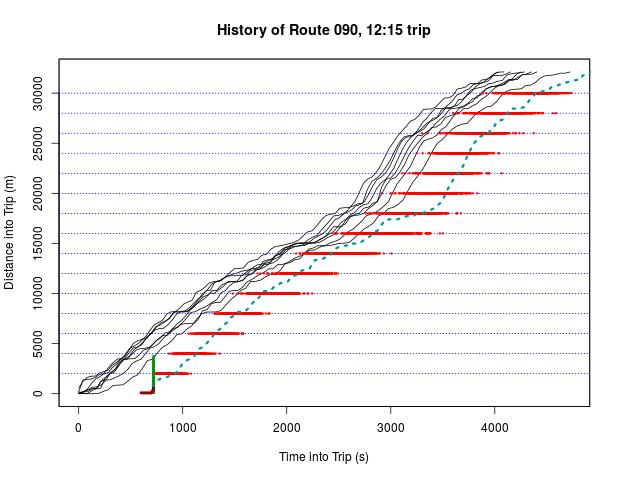
\includegraphics[width=\textwidth]{hist/route090_1215_001.jpg}
    \label{fig:route090-history-1}
  \end{subfigure}%
  \begin{subfigure}{0.33\textwidth}
    \centering
    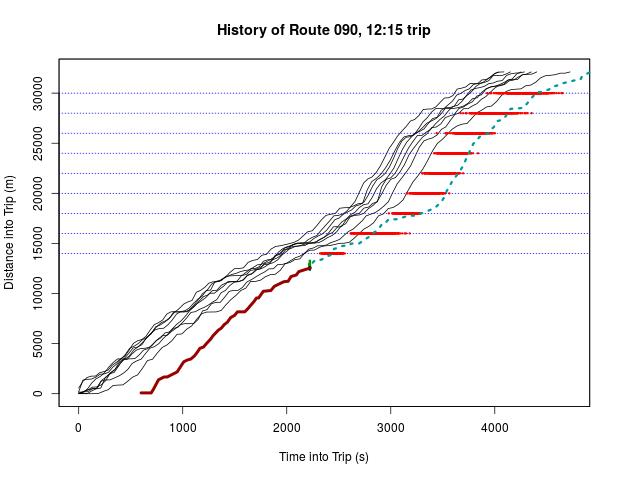
\includegraphics[width=\textwidth]{hist/route090_1215_040.jpg}
    \label{fig:route090-history-2}
  \end{subfigure}%
  \begin{subfigure}{0.33\textwidth}  
    \centering
    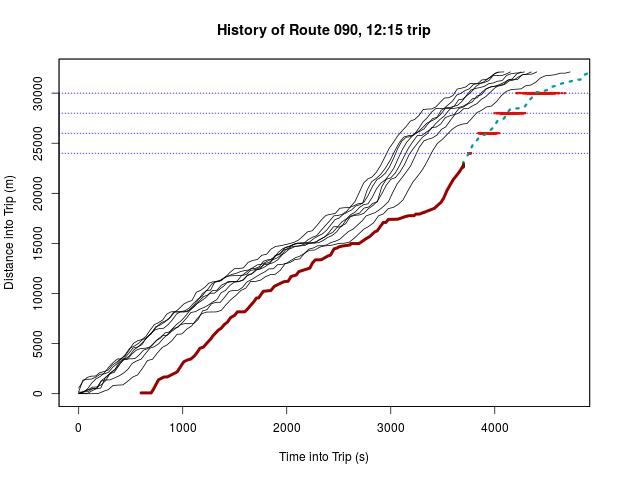
\includegraphics[width=\textwidth]{hist/route090_1215_081.jpg}
    \label{fig:route090-history-3}
  \end{subfigure}
  \caption{Arrival time predictions for a single route, using only historical data.}
  \label{fig:route090-history}
\end{figure}


There we have it. Here's a summary:
\begin{itemize}
\item Predicions only use historical data
\item Each particle is used to make an individual prediction, based on
  the \emph{distribution} of time taken to get to the stop in
  historical trips.
\item the \emph{distribution} is of time taken for particle $i$ to get
  from distance $d_k(i)$ to stop $s_j$ is $t_{k,j}(i)$ is normally distributed.
\end{itemize}



There are several directions we can go from here:
\begin{itemize}
\item using dynamic motion to adjust predictions (i.e., velocity and acceleration)
\item similar to above, but weight historical trips based on
  \emph{velocity} at the current distance, or distance/speed at current time.
\item \textbf{use multiple \emph{trips} and weight based on how old they are,
  and maybe some historical correlation between trips.}
\end{itemize}


We're going to go with the last option first, because its moreorless
what we want to focus our attentions on.




\section{Using Multiple Trips}
\label{sec:multiple_trips}

The ``raw'' data is:

\begin{knitrout}
\definecolor{shadecolor}{rgb}{0.969, 0.969, 0.969}\color{fgcolor}\begin{kframe}
\begin{alltt}
\hlkwd{with}\hlstd{(hist090,} \hlkwd{plot}\hlstd{(time.hour, distance,} \hlkwc{type} \hlstd{=} \hlstr{"n"}\hlstd{,}
                   \hlkwc{main} \hlstd{=} \hlstr{"History of Route 090"}\hlstd{,} \hlkwc{xlab} \hlstd{=} \hlstr{"Time (h)"}\hlstd{,}
                   \hlkwc{ylab} \hlstd{=} \hlstr{"Distance into Trip (m)"}\hlstd{))}
\hlkwd{invisible}\hlstd{(}\hlkwd{tapply}\hlstd{(}\hlnum{1}\hlopt{:}\hlkwd{nrow}\hlstd{(hist090), hist090}\hlopt{$}\hlstd{dvt,}
                 \hlkwa{function}\hlstd{(}\hlkwc{i}\hlstd{)} \hlkwd{lines}\hlstd{(hist090}\hlopt{$}\hlstd{time.hour[i], hist090}\hlopt{$}\hlstd{distance[i])))}
\end{alltt}
\end{kframe}
\includegraphics[width=\maxwidth]{figure/multiple_route_history-1} 

\end{knitrout}

To get an idea of relatedness between trips, we'll zero them all, and stuff.

\begin{knitrout}
\definecolor{shadecolor}{rgb}{0.969, 0.969, 0.969}\color{fgcolor}\begin{kframe}
\begin{alltt}
\hlstd{hist090}\hlopt{$}\hlstd{dvt} \hlkwb{<-} \hlkwd{factor}\hlstd{(hist090}\hlopt{$}\hlstd{dvt)}
\hlstd{hist090}\hlopt{$}\hlstd{time.zero} \hlkwb{<-}
    \hlkwd{do.call}\hlstd{(c,} \hlkwd{tapply}\hlstd{(}\hlnum{1}\hlopt{:}\hlkwd{nrow}\hlstd{(hist090), hist090}\hlopt{$}\hlstd{dvt,}
                      \hlkwa{function}\hlstd{(}\hlkwc{i}\hlstd{) hist090}\hlopt{$}\hlstd{time.day[i]} \hlopt{-} \hlkwd{min}\hlstd{(hist090}\hlopt{$}\hlstd{time.day[i])))}
\hlstd{trip.starttime} \hlkwb{<-} \hlkwd{tapply}\hlstd{(hist090}\hlopt{$}\hlstd{time.day, hist090}\hlopt{$}\hlstd{dvt, min)}
\hlstd{coli} \hlkwb{<-} \hlkwa{function}\hlstd{(}\hlkwc{t}\hlstd{,} \hlkwc{r} \hlstd{=} \hlkwd{range}\hlstd{(tnum),} \hlkwc{tnum} \hlstd{=} \hlkwd{as.numeric}\hlstd{(t))}
    \hlkwd{structure}\hlstd{(}\hlkwd{rainbow}\hlstd{(}\hlnum{101}\hlstd{)[}\hlkwd{round}\hlstd{((tnum} \hlopt{-} \hlkwd{min}\hlstd{(r))} \hlopt{/} \hlkwd{diff}\hlstd{(r)} \hlopt{*} \hlnum{100}\hlstd{)} \hlopt{+} \hlnum{1}\hlstd{],}
              \hlkwc{.Names} \hlstd{=} \hlkwd{names}\hlstd{(t))}
\hlstd{hist090}\hlopt{$}\hlstd{colour} \hlkwb{<-} \hlkwd{as.character}\hlstd{(}\hlkwd{coli}\hlstd{(trip.starttime)[hist090}\hlopt{$}\hlstd{dvt])}


\hlkwd{with}\hlstd{(hist090,} \hlkwd{plot}\hlstd{(time.zero, distance,} \hlkwc{type} \hlstd{=} \hlstr{"n"}\hlstd{,}
                   \hlkwc{main} \hlstd{=} \hlstr{"History of Route 090"}\hlstd{,} \hlkwc{xlab} \hlstd{=} \hlstr{"Time into Trip (s)"}\hlstd{,}
                   \hlkwc{ylab} \hlstd{=} \hlstr{"Distance into Trip (m)"}\hlstd{))}
\hlkwd{invisible}\hlstd{(}\hlkwd{tapply}\hlstd{(}\hlnum{1}\hlopt{:}\hlkwd{nrow}\hlstd{(hist090), hist090}\hlopt{$}\hlstd{dvt,}
                 \hlkwa{function}\hlstd{(}\hlkwc{i}\hlstd{)} \hlkwd{lines}\hlstd{(hist090}\hlopt{$}\hlstd{time.zero[i], hist090}\hlopt{$}\hlstd{distance[i],}
                                   \hlkwc{col} \hlstd{= hist090}\hlopt{$}\hlstd{colour[i[}\hlnum{1}\hlstd{]])))}
\end{alltt}
\end{kframe}
\includegraphics[width=\maxwidth]{figure/comparing_multiple_trips-1} 

\end{knitrout}


That looks nice, but it's not all that useful.
We want $(\Delta d)_{d,\delta}$, 
the \emph{distance traveled} from distance $d$~m into trip in $\delta$~seconds.
That is,
\begin{equation}
  \label{eq:predict-distance}
  \Ex{d_k(i)} = d_{k-1}(i) + \Ex{(\Delta d)_{d_{k-1},t_k}}.
\end{equation}
However, previously $(\Delta d)_{d,\delta}$ was distributed normally,
with mean and standard deviation obtained from historical data, i.e.,
$\Ex{(\Delta d)_{d_{k-1},t_k}\given D_{j,r}}, j = \{1,...,J-1\}, r = \text{current trip ID}$ and $J$
the current ``day''.
Now, we want to introduce a probability $\phi$, the ``correlation'' between two successive trips.
We will use the time taken by the previous trip (along the same route), $r-1$,
with probability $\phi_k$, otherwise use the expected value above.

Defining $a_{d,j,r} = a(d\given j, r)$ as the arrival time at some arbitrary distance $d$ 
(a future stop, or current location), on day $j$, trip $r$,
the distance traveled from $d_1$ in $\delta$ seconds is:
\begin{equation}
  \label{eq:previous_trip_delta}
  (\Delta d)_{d_1,\delta}\given D_{j,r-1} =
  a^{-1}(a_{d_1,j, r-1} + \delta\given j,r-1)
\end{equation}

Essentially, $a$ is the inverse of the fitted bus trajectory, $d(t\given j,r)$.
So (\ref{eq:previous_trip_delta}) becomes
\begin{equation}
  \label{eq:previous_trip_delta_2}
  (\Delta d)_{d_1,\delta}\given D_{j,r-1} =
  d(a_{d_1,j, r-1} + \delta\given j,r-1).
\end{equation}


Well that's not confusing at all.

So, basically, the above equations work for anything (historical, previous routes, etc).
Now, the expected distance is:
\begin{equation}
  \label{eq:expected_hist_prev_}
   \Ex{d_k(i)} = d_{k-1}(i) +
   \begin{cases}
     (\Delta d)_{d_1,\delta}\given D_{j,r-1} & \text{w.p. } \phi_k(i), \\
      \Ex{(\Delta d)_{d_{k-1},t_k}} & \text{w.p. } 1 - \phi_k(i)
   \end{cases}.
\end{equation}
For the variance, we'll just use the variance at that point \ldots


\begin{knitrout}
\definecolor{shadecolor}{rgb}{0.969, 0.969, 0.969}\color{fgcolor}\begin{kframe}
\begin{alltt}
\hlcom{## the trips}
\hlstd{R} \hlkwb{<-} \hlkwd{unique}\hlstd{(}\hlkwd{gsub}\hlstd{(}\hlstr{"-.+$"}\hlstd{,} \hlstr{""}\hlstd{, hist090}\hlopt{$}\hlstd{trip_id))}
\hlcom{## start times}
\hlstd{R.start} \hlkwb{<-} \hlkwd{sapply}\hlstd{(R,} \hlkwa{function}\hlstd{(}\hlkwc{r}\hlstd{)}
    \hlstd{hist090[}\hlkwd{grepl}\hlstd{(r, hist090}\hlopt{$}\hlstd{trip_id),} \hlstr{"trip_start_time"}\hlstd{][}\hlnum{1}\hlstd{])}

\hlstd{r} \hlkwb{<-} \hlstr{"3090020609"}

\hlstd{hist} \hlkwb{<-} \hlstd{hist090[}\hlkwd{grepl}\hlstd{(tripid, hist090}\hlopt{$}\hlstd{trip_id), ]}
\hlstd{hist}\hlopt{$}\hlstd{dvt} \hlkwb{<-} \hlkwd{factor}\hlstd{(hist}\hlopt{$}\hlstd{dvt)}
\hlstd{hist}\hlopt{$}\hlstd{time_into_trip} \hlkwb{<-}
    \hlkwd{do.call}\hlstd{(c,} \hlkwd{tapply}\hlstd{(}\hlnum{1}\hlopt{:}\hlkwd{nrow}\hlstd{(hist), hist}\hlopt{$}\hlstd{dvt,}
                      \hlkwa{function}\hlstd{(}\hlkwc{i}\hlstd{) hist}\hlopt{$}\hlstd{time.day[i]} \hlopt{-} \hlkwd{min}\hlstd{(hist}\hlopt{$}\hlstd{time.day[i])))}

\hlstd{test.trip} \hlkwb{<-} \hlstd{hist[hist}\hlopt{$}\hlstd{trip_start_date} \hlopt{==} \hlkwd{tail}\hlstd{(}\hlkwd{unique}\hlstd{(hist}\hlopt{$}\hlstd{trip_start_date),} \hlnum{1}\hlstd{), ]}
\hlstd{hist} \hlkwb{<-} \hlstd{hist[hist}\hlopt{$}\hlstd{trip_start_date} \hlopt{!=} \hlkwd{tail}\hlstd{(}\hlkwd{unique}\hlstd{(hist}\hlopt{$}\hlstd{trip_start_date),} \hlnum{1}\hlstd{), ]}
\hlstd{hist}\hlopt{$}\hlstd{dvt} \hlkwb{<-} \hlkwd{factor}\hlstd{(hist}\hlopt{$}\hlstd{dvt)}

\hlcom{## previous trip on test day}
\hlstd{rtimes} \hlkwb{<-} \hlkwd{sort}\hlstd{(}\hlkwd{unique}\hlstd{(hist090[hist090}\hlopt{$}\hlstd{trip_start_date} \hlopt{==}
                              \hlstd{test.trip}\hlopt{$}\hlstd{trip_start_date[}\hlnum{1}\hlstd{],}
                              \hlstr{"trip_start_time"}\hlstd{]))}
\hlstd{ri} \hlkwb{<-} \hlkwd{which}\hlstd{(rtimes} \hlopt{==} \hlstd{test.trip}\hlopt{$}\hlstd{trip_start_time[}\hlnum{1}\hlstd{])}
\hlstd{rpred} \hlkwb{<-} \hlstd{hist090[hist090}\hlopt{$}\hlstd{trip_start_time} \hlopt{==} \hlstd{rtimes[ri} \hlopt{-} \hlnum{1}\hlstd{]} \hlopt{&}
                 \hlstd{hist090}\hlopt{$}\hlstd{trip_start_date} \hlopt{==} \hlstd{test.trip}\hlopt{$}\hlstd{trip_start_date[}\hlnum{1}\hlstd{], ]}

\hlkwd{with}\hlstd{(hist,} \hlkwd{plot}\hlstd{(time_into_trip, distance,} \hlkwc{type} \hlstd{=} \hlstr{"n"}\hlstd{,}
                \hlkwc{main} \hlstd{=} \hlstr{"History of Route 090 12:15 trip and Previous 11:15 trip"}\hlstd{,}
                \hlkwc{xlab} \hlstd{=} \hlstr{"Time into Trip (s)"}\hlstd{,}
                \hlkwc{ylab} \hlstd{=} \hlstr{"Distance into Trip (m)"}\hlstd{))}
\hlkwd{invisible}\hlstd{(}\hlkwd{tapply}\hlstd{(}\hlnum{1}\hlopt{:}\hlkwd{nrow}\hlstd{(hist), hist}\hlopt{$}\hlstd{dvt,}
                 \hlkwa{function}\hlstd{(}\hlkwc{i}\hlstd{)} \hlkwd{lines}\hlstd{(hist}\hlopt{$}\hlstd{time_into_trip[i], hist}\hlopt{$}\hlstd{distance[i])))}

\hlstd{stops} \hlkwb{<-} \hlnum{1}\hlopt{:}\hlnum{15} \hlopt{*} \hlnum{2000}
\hlkwd{abline}\hlstd{(}\hlkwc{h} \hlstd{=} \hlkwd{c}\hlstd{(}\hlnum{0}\hlstd{, stops),} \hlkwc{col} \hlstd{=} \hlstr{"#0000ff"}\hlstd{,} \hlkwc{lty} \hlstd{=} \hlnum{3}\hlstd{)}

\hlkwd{with}\hlstd{(rpred,} \hlkwd{lines}\hlstd{(time.zero} \hlopt{+} \hlnum{10}\hlopt{*}\hlnum{60}\hlstd{, distance,} \hlkwc{col} \hlstd{=} \hlstr{"#990000"}\hlstd{,} \hlkwc{lwd} \hlstd{=} \hlnum{2}\hlstd{))}
\hlkwd{with}\hlstd{(test.trip,} \hlkwd{lines}\hlstd{(time.zero} \hlopt{+} \hlnum{10}\hlopt{*}\hlnum{60}\hlstd{, distance,} \hlkwc{col} \hlstd{=} \hlstr{"#009900"}\hlstd{,} \hlkwc{lwd} \hlstd{=} \hlnum{2}\hlstd{,} \hlkwc{lty} \hlstd{=} \hlnum{3}\hlstd{))}
\end{alltt}
\end{kframe}
\includegraphics[width=\maxwidth]{figure/historical_sameday-1} 

\end{knitrout}


\begin{knitrout}
\definecolor{shadecolor}{rgb}{0.969, 0.969, 0.969}\color{fgcolor}\begin{kframe}
\begin{alltt}
\hlstd{rpred.fn} \hlkwb{<-} \hlkwd{try}\hlstd{(\{}
    \hlstd{f}\hlkwb{=}\hlkwd{splinefun}\hlstd{(rpred}\hlopt{$}\hlstd{time.zero, rpred}\hlopt{$}\hlstd{distance,}
                \hlkwc{method} \hlstd{=} \hlstr{"hyman"}\hlstd{,} \hlkwc{ties} \hlstd{= min)}
    \hlkwd{attr}\hlstd{(f,} \hlstr{"max"}\hlstd{)} \hlkwb{<-} \hlkwd{max}\hlstd{(rpred}\hlopt{$}\hlstd{time.zero)}
    \hlstd{f}
\hlstd{\},} \hlkwc{silent} \hlstd{=} \hlnum{TRUE}\hlstd{)}
\hlstd{.predarrivalTime} \hlkwb{<-} \hlkwa{function}\hlstd{(}\hlkwc{d}\hlstd{)}
    \hlkwd{optimize}\hlstd{(}\hlkwa{function}\hlstd{(}\hlkwc{x}\hlstd{) (}\hlkwd{rpred.fn}\hlstd{(x)} \hlopt{-} \hlstd{d)}\hlopt{^}\hlnum{2}\hlstd{,}
             \hlkwc{interval} \hlstd{=} \hlkwd{range}\hlstd{(rpred}\hlopt{$}\hlstd{time.zero))}\hlopt{$}\hlstd{minimum}
\hlstd{predarrivalTime} \hlkwb{<-} \hlkwd{Vectorize}\hlstd{(.predarrivalTime,} \hlstr{"d"}\hlstd{)}
\hlstd{.predhistory.fnD} \hlkwb{<-} \hlkwa{function}\hlstd{(}\hlkwc{d}\hlstd{,} \hlkwc{delta} \hlstd{=} \hlnum{0}\hlstd{,} \hlkwc{deriv} \hlstd{=} \hlnum{0}\hlstd{) \{}
    \hlcom{## convert distance to time, time to ["speed", "acceleration"]}
    \hlstd{t} \hlkwb{<-} \hlkwd{optimize}\hlstd{(}
        \hlkwa{function}\hlstd{(}\hlkwc{x}\hlstd{) (}\hlkwd{rpred.fn}\hlstd{(x)} \hlopt{-} \hlstd{d)}\hlopt{^}\hlnum{2}\hlstd{,}
        \hlkwc{interval} \hlstd{=} \hlkwd{range}\hlstd{(hist}\hlopt{$}\hlstd{time_into_trip)}
    \hlstd{)}\hlopt{$}\hlstd{minimum}
    \hlkwd{rpred.fn}\hlstd{(t} \hlopt{+} \hlstd{delta,} \hlkwc{deriv} \hlstd{= deriv)}
\hlstd{\}}
\hlstd{predhistory.fnD} \hlkwb{<-} \hlkwd{Vectorize}\hlstd{(.predhistory.fnD,} \hlstr{"d"}\hlstd{)}

\hlstd{draw} \hlkwb{<-} \hlkwa{function}\hlstd{(}\hlkwc{s} \hlstd{=} \hlnum{0}\hlstd{,} \hlkwc{a}\hlstd{,} \hlkwc{labs} \hlstd{=} \hlnum{TRUE}\hlstd{,} \hlkwc{xlim} \hlstd{=} \hlkwa{NULL}\hlstd{,} \hlkwc{ylim} \hlstd{=} \hlkwa{NULL}\hlstd{,}
                 \hlkwc{stop.pch} \hlstd{=} \hlnum{19}\hlstd{,} \hlkwc{stop.col} \hlstd{=} \hlstr{"red"}\hlstd{) \{}
    \hlkwd{with}\hlstd{(hist,} \hlkwd{plot}\hlstd{(time_into_trip, distance,} \hlkwc{type} \hlstd{=} \hlstr{"n"}\hlstd{,}
                    \hlkwc{main} \hlstd{=} \hlkwd{ifelse}\hlstd{(}
                        \hlstd{labs,}
                        \hlstr{"History of Route 090, 12:15 trip and previous 11:15 trip"}\hlstd{,}
                        \hlstr{""}\hlstd{),}
                    \hlkwc{xlab} \hlstd{=} \hlkwd{ifelse}\hlstd{(labs,} \hlstr{"Time into Trip (s)"}\hlstd{,} \hlstr{""}\hlstd{),}
                    \hlkwc{ylab} \hlstd{=} \hlkwd{ifelse}\hlstd{(labs,} \hlstr{"Distance into Trip (m)"}\hlstd{,} \hlstr{""}\hlstd{),}
                    \hlkwc{xlim} \hlstd{= xlim,} \hlkwc{ylim} \hlstd{= ylim,}
                    \hlkwc{axes} \hlstd{= labs))}
    \hlkwd{box}\hlstd{()}
    \hlkwd{invisible}\hlstd{(}\hlkwd{lapply}\hlstd{(history.fn,} \hlkwa{function}\hlstd{(}\hlkwc{f}\hlstd{)}
        \hlkwd{curve}\hlstd{(}\hlkwd{f}\hlstd{(x),} \hlnum{0}\hlstd{,} \hlkwd{attr}\hlstd{(f,} \hlstr{"max"}\hlstd{),} \hlkwc{n} \hlstd{=} \hlnum{101}\hlstd{,} \hlkwc{add} \hlstd{=} \hlnum{TRUE}\hlstd{,} \hlkwc{lty} \hlstd{=} \hlnum{2}\hlstd{)))}
    \hlkwd{curve}\hlstd{(}\hlkwd{rpred.fn}\hlstd{(x} \hlopt{-} \hlnum{600}\hlstd{),} \hlnum{600}\hlstd{,} \hlkwd{attr}\hlstd{(rpred.fn,} \hlstr{"max"}\hlstd{)} \hlopt{+} \hlnum{600}\hlstd{,}
          \hlkwc{n} \hlstd{=} \hlnum{101}\hlstd{,} \hlkwc{add} \hlstd{=} \hlnum{TRUE}\hlstd{,} \hlkwc{col} \hlstd{=} \hlstr{"#990000"}\hlstd{,} \hlkwc{lwd} \hlstd{=} \hlnum{3}\hlstd{)}
    \hlkwa{if} \hlstd{(}\hlkwd{any}\hlstd{(s} \hlopt{==} \hlnum{0}\hlstd{))}
        \hlkwd{abline}\hlstd{(}\hlkwc{h} \hlstd{=} \hlkwd{c}\hlstd{(}\hlnum{0}\hlstd{, stops),} \hlkwc{col} \hlstd{=} \hlstr{"#0000ff"}\hlstd{,} \hlkwc{lty} \hlstd{=} \hlnum{3}\hlstd{)}
    \hlkwa{else if} \hlstd{(}\hlkwd{all}\hlstd{(s} \hlopt{>} \hlnum{0}\hlstd{))}
        \hlkwd{abline}\hlstd{(}\hlkwc{h} \hlstd{= stops[s],} \hlkwc{col} \hlstd{=} \hlstr{"#0000ff"}\hlstd{,} \hlkwc{lty} \hlstd{=} \hlnum{3}\hlstd{)}

    \hlkwa{if} \hlstd{(}\hlopt{!}\hlkwd{missing}\hlstd{(a)} \hlopt{&&} \hlkwd{all}\hlstd{(s} \hlopt{>} \hlnum{0}\hlstd{)) \{}
        \hlkwa{if} \hlstd{(}\hlopt{!}\hlkwd{is.matrix}\hlstd{(a)) a} \hlkwb{<-} \hlkwd{rbind}\hlstd{(a)}
        \hlkwa{if} \hlstd{(}\hlkwd{length}\hlstd{(s)} \hlopt{==} \hlkwd{nrow}\hlstd{(a)) \{}
            \hlkwa{for} \hlstd{(i} \hlkwa{in} \hlnum{1}\hlopt{:}\hlkwd{nrow}\hlstd{(a))}
                \hlkwd{points}\hlstd{(a[i, ],} \hlkwd{rep}\hlstd{(stops[s[i]],} \hlkwd{ncol}\hlstd{(a)),}
                       \hlkwc{pch} \hlstd{= stop.pch,} \hlkwc{col} \hlstd{= stop.col,} \hlkwc{cex} \hlstd{=} \hlnum{0.3}\hlstd{)}
        \hlstd{\}}
    \hlstd{\}}
\hlstd{\}}

\hlcom{## convert w from before into an array (2 x M x N = parameters x particles x obs)}
\hlstd{N} \hlkwb{<-} \hlkwd{nrow}\hlstd{(test.trip)}
\hlstd{w} \hlkwb{<-} \hlkwd{array}\hlstd{(}\hlnum{NA}\hlstd{,} \hlkwc{dim} \hlstd{=} \hlkwd{c}\hlstd{(}\hlnum{2}\hlstd{, M, N))}
\hlstd{w[}\hlnum{1}\hlstd{,,}\hlnum{1}\hlstd{]} \hlkwb{<-} \hlnum{0} \hlcom{## start position is 0}
\hlstd{w[}\hlnum{2}\hlstd{,,}\hlnum{1}\hlstd{]} \hlkwb{<-} \hlkwd{runif}\hlstd{(M)} \hlcom{## start correlation is ~ U[0,1]}
\hlstd{w0} \hlkwb{<-} \hlstd{w}  \hlcom{## matrix for the original estimates}

\hlstd{test.trip}\hlopt{$}\hlstd{time_into_trip} \hlkwb{<-} \hlstd{test.trip}\hlopt{$}\hlstd{time_into_trip} \hlopt{+} \hlnum{600}
\hlstd{t} \hlkwb{<-} \hlstd{test.trip}\hlopt{$}\hlstd{time_into_trip}
\hlstd{delta.t} \hlkwb{<-} \hlkwd{c}\hlstd{(}\hlnum{0}\hlstd{,} \hlkwd{diff}\hlstd{(t))}

\hlstd{pred1} \hlkwb{<-} \hlkwd{history.fnD}\hlstd{(w[}\hlnum{1}\hlstd{,,}\hlnum{1}\hlstd{], delta.t[}\hlnum{2}\hlstd{])}
\hlstd{pred2} \hlkwb{<-} \hlkwd{predhistory.fnD}\hlstd{(w[}\hlnum{1}\hlstd{,,}\hlnum{1}\hlstd{], delta.t[}\hlnum{2}\hlstd{])}
\hlstd{w0[}\hlnum{2}\hlstd{,,}\hlnum{2}\hlstd{]} \hlkwb{<-} \hlkwd{pnorm}\hlstd{(}\hlkwd{qnorm}\hlstd{(w[}\hlnum{2}\hlstd{,,}\hlnum{1}\hlstd{])} \hlopt{+} \hlkwd{rnorm}\hlstd{(M))}
\hlstd{w0[}\hlnum{1}\hlstd{,,}\hlnum{2}\hlstd{]} \hlkwb{<-} \hlkwd{rtnorm}\hlstd{(M,} \hlkwd{ifelse}\hlstd{(}\hlkwd{runif}\hlstd{(M)} \hlopt{<} \hlstd{w0[}\hlnum{2}\hlstd{,,}\hlnum{2}\hlstd{],}
                             \hlkwd{colMeans}\hlstd{(pred1),}
                             \hlstd{pred2),}
                   \hlkwd{apply}\hlstd{(pred1,} \hlnum{2}\hlstd{, sd),} \hlkwc{lower} \hlstd{= w[}\hlnum{1}\hlstd{,,}\hlnum{1}\hlstd{])}
\hlstd{Pi} \hlkwb{<-} \hlkwd{dnorm}\hlstd{(w0[}\hlnum{1}\hlstd{,,}\hlnum{2}\hlstd{], test.trip}\hlopt{$}\hlstd{distance[}\hlnum{2}\hlstd{],} \hlnum{20}\hlstd{)}
\hlstd{wi} \hlkwb{<-} \hlstd{Pi} \hlopt{/} \hlkwd{sum}\hlstd{(Pi)}
\hlstd{w[,,}\hlnum{2}\hlstd{]} \hlkwb{<-} \hlstd{w0[,} \hlkwd{sample}\hlstd{(M,} \hlkwc{replace} \hlstd{=} \hlnum{TRUE}\hlstd{,} \hlkwc{prob} \hlstd{= wi),} \hlnum{2}\hlstd{]}
\hlkwd{draw}\hlstd{()}
\hlkwd{with}\hlstd{(test.trip,} \hlkwd{lines}\hlstd{(time_into_trip[}\hlnum{1}\hlopt{:}\hlnum{2}\hlstd{], distance[}\hlnum{1}\hlopt{:}\hlnum{2}\hlstd{],}
                      \hlkwc{col} \hlstd{=} \hlstr{"#000099"}\hlstd{,} \hlkwc{lwd} \hlstd{=} \hlnum{4}\hlstd{))}
\hlkwd{with}\hlstd{(test.trip,} \hlkwd{lines}\hlstd{(time_into_trip[}\hlopt{-}\hlstd{(}\hlnum{1}\hlopt{:}\hlnum{2}\hlstd{)], distance[}\hlopt{-}\hlstd{(}\hlnum{1}\hlopt{:}\hlnum{2}\hlstd{)],}
                      \hlkwc{col} \hlstd{=} \hlstr{"#009999"}\hlstd{,} \hlkwc{lwd} \hlstd{=} \hlnum{3}\hlstd{,} \hlkwc{lty} \hlstd{=} \hlnum{3}\hlstd{))}

\hlkwd{points}\hlstd{(}\hlkwd{rep}\hlstd{(t[}\hlnum{2}\hlstd{], M), w0[}\hlnum{1}\hlstd{,,}\hlnum{2}\hlstd{],} \hlkwc{col} \hlstd{=} \hlstr{"#009900"}\hlstd{,} \hlkwc{pch} \hlstd{=} \hlnum{19}\hlstd{,} \hlkwc{cex} \hlstd{=} \hlnum{0.3}\hlstd{)}
\hlkwd{points}\hlstd{(}\hlkwd{rep}\hlstd{(t[}\hlnum{2}\hlstd{], M), w[}\hlnum{1}\hlstd{,,}\hlnum{2}\hlstd{],} \hlkwc{col} \hlstd{=} \hlstr{"magenta"}\hlstd{,} \hlkwc{pch} \hlstd{=} \hlnum{19}\hlstd{,} \hlkwc{cex} \hlstd{=} \hlnum{0.3}\hlstd{)}
\end{alltt}
\end{kframe}
\includegraphics[width=\maxwidth]{figure/supporting_functions-1} 

\end{knitrout}




\begin{knitrout}
\definecolor{shadecolor}{rgb}{0.969, 0.969, 0.969}\color{fgcolor}\begin{kframe}
\begin{alltt}
\hlstd{predict} \hlkwb{<-} \hlkwa{function}\hlstd{(}\hlkwc{i}\hlstd{,} \hlkwc{draw} \hlstd{=} \hlnum{TRUE}\hlstd{,} \hlkwc{...}\hlstd{) \{}
    \hlstd{pred1} \hlkwb{<-} \hlkwd{history.fnD}\hlstd{(w[}\hlnum{1}\hlstd{,,i}\hlopt{-}\hlnum{1}\hlstd{], delta.t[i])}
    \hlstd{pred2} \hlkwb{<-} \hlkwd{predhistory.fnD}\hlstd{(w[}\hlnum{1}\hlstd{,,i}\hlopt{-}\hlnum{1}\hlstd{], delta.t[i])}
    \hlstd{w0[}\hlnum{2}\hlstd{,,i]} \hlkwb{<-} \hlkwd{pnorm}\hlstd{(}\hlkwd{qnorm}\hlstd{(w[}\hlnum{2}\hlstd{,,i}\hlopt{-}\hlnum{1}\hlstd{])} \hlopt{+} \hlkwd{rnorm}\hlstd{(M))}
    \hlstd{w0[}\hlnum{1}\hlstd{,,i]} \hlkwb{<-} \hlkwd{rtnorm}\hlstd{(M,} \hlkwd{ifelse}\hlstd{(}\hlkwd{runif}\hlstd{(M)} \hlopt{>} \hlstd{w0[}\hlnum{2}\hlstd{,,i],}
                                 \hlkwd{colMeans}\hlstd{(pred1),}
                                 \hlstd{pred2),}
                       \hlkwd{apply}\hlstd{(pred1,} \hlnum{2}\hlstd{, sd),} \hlkwc{lower} \hlstd{= w[}\hlnum{1}\hlstd{,,i}\hlopt{-}\hlnum{1}\hlstd{])}
    \hlstd{Pi} \hlkwb{<-} \hlkwd{dnorm}\hlstd{(w0[}\hlnum{1}\hlstd{,,i], test.trip}\hlopt{$}\hlstd{distance[i],} \hlnum{20}\hlstd{)}
    \hlkwa{if} \hlstd{(}\hlkwd{sum}\hlstd{(Pi)} \hlopt{==} \hlnum{0}\hlstd{) \{}
        \hlstd{w0[ , , i]} \hlkwb{<-} \hlkwd{runif}\hlstd{(M,} \hlnum{0}\hlstd{,} \hlkwc{max} \hlstd{=} \hlkwd{max}\hlstd{(w0[, , i]))}
        \hlstd{Pi} \hlkwb{<-} \hlkwd{dnorm}\hlstd{(w0[}\hlnum{1}\hlstd{,,i], test.trip}\hlopt{$}\hlstd{distance[i],} \hlnum{20}\hlstd{)}
        \hlkwa{if} \hlstd{(}\hlkwd{sum}\hlstd{(Pi)} \hlopt{==} \hlnum{0}\hlstd{) \{}
            \hlstd{w0[ , , i]} \hlkwb{<-} \hlkwd{runif}\hlstd{(M,} \hlnum{0}\hlstd{,} \hlkwc{max} \hlstd{=} \hlnum{2} \hlopt{*} \hlkwd{max}\hlstd{(w0[, , i]))}
            \hlstd{Pi} \hlkwb{<-} \hlkwd{dnorm}\hlstd{(w0[}\hlnum{1}\hlstd{,,i], test.trip}\hlopt{$}\hlstd{distance[i],} \hlnum{20}\hlstd{)}
        \hlstd{\}}
    \hlstd{\}}
    \hlstd{wi} \hlkwb{<-} \hlstd{Pi} \hlopt{/} \hlkwd{sum}\hlstd{(Pi)}
    \hlstd{w[,,i]} \hlkwb{<<-} \hlstd{w0[,} \hlkwd{sample}\hlstd{(M,} \hlkwc{replace} \hlstd{=} \hlnum{TRUE}\hlstd{,} \hlkwc{prob} \hlstd{= wi), i]}

    \hlstd{wstops} \hlkwb{<-} \hlkwd{which}\hlstd{(stops} \hlopt{>} \hlkwd{min}\hlstd{(w[}\hlnum{1}\hlstd{,,i]))}
    \hlstd{stops} \hlkwb{<-} \hlstd{stops[wstops]}
    \hlstd{a} \hlkwb{<-} \hlkwd{matrix}\hlstd{(}\hlkwc{nrow} \hlstd{=} \hlkwd{length}\hlstd{(stops),} \hlkwc{ncol} \hlstd{= M)}
    \hlstd{ti} \hlkwb{<-} \hlstd{test.trip}\hlopt{$}\hlstd{time_into_trip[i]}
    \hlstd{USE} \hlkwb{<-} \hlkwd{runif}\hlstd{(M)} \hlopt{<} \hlstd{w[}\hlnum{2}\hlstd{,,i]}
    \hlstd{a1j} \hlkwb{<-} \hlkwd{arrivalTime}\hlstd{(stops[}\hlnum{1}\hlstd{])[,}\hlnum{1}\hlstd{]}
    \hlstd{adj} \hlkwb{<-} \hlopt{-} \hlkwd{sweep}\hlstd{(}\hlkwd{arrivalTime}\hlstd{(w[}\hlnum{1}\hlstd{,,i]),} \hlnum{1}\hlstd{, a1j)}
    \hlstd{adj[adj} \hlopt{<} \hlnum{0}\hlstd{]} \hlkwb{<-} \hlnum{0}
    \hlstd{adpred} \hlkwb{<-} \hlkwd{predarrivalTime}\hlstd{(stops[}\hlnum{1}\hlstd{])} \hlopt{-} \hlkwd{predarrivalTime}\hlstd{(w[}\hlnum{1}\hlstd{,,i])}
    \hlstd{a[}\hlnum{1}\hlstd{, ]} \hlkwb{<-} \hlstd{ti} \hlopt{+} \hlkwd{rtnorm}\hlstd{(M,} \hlkwd{ifelse}\hlstd{(}\hlopt{!}\hlstd{USE,}
                                    \hlkwd{colMeans}\hlstd{(adj),}
                                    \hlkwd{rep}\hlstd{(adpred, M)),}
                          \hlkwd{pmax}\hlstd{(}\hlnum{1}\hlstd{,} \hlkwd{colSds}\hlstd{(adj)),} \hlkwc{lower} \hlstd{=} \hlnum{0}\hlstd{)}

    \hlkwa{for} \hlstd{(j} \hlkwa{in} \hlnum{2}\hlopt{:}\hlkwd{length}\hlstd{(stops)) \{}
        \hlstd{ajj} \hlkwb{<-} \hlkwd{arrivalTime}\hlstd{(stops[j])[,}\hlnum{1}\hlstd{]}
        \hlstd{adj} \hlkwb{<-} \hlopt{-} \hlkwd{sweep}\hlstd{(}\hlkwd{arrivalTime}\hlstd{(w[}\hlnum{1}\hlstd{,,i]),} \hlnum{1}\hlstd{, ajj)}
        \hlstd{adj[adj} \hlopt{<} \hlnum{0}\hlstd{]} \hlkwb{<-} \hlnum{0}
        \hlstd{adpred} \hlkwb{<-} \hlkwd{predarrivalTime}\hlstd{(stops[j])} \hlopt{-} \hlkwd{predarrivalTime}\hlstd{(w[}\hlnum{1}\hlstd{,,i])}
        \hlstd{a[j, ]} \hlkwb{<-} \hlstd{ti} \hlopt{+} \hlkwd{rtnorm}\hlstd{(M,} \hlkwd{ifelse}\hlstd{(}\hlopt{!}\hlstd{USE,}
                                        \hlkwd{colMeans}\hlstd{(adj),}
                                        \hlkwd{rep}\hlstd{(adpred, M)),}
                              \hlkwd{pmax}\hlstd{(}\hlnum{1}\hlstd{,} \hlkwd{colSds}\hlstd{(adj)),} \hlkwc{lower} \hlstd{=} \hlnum{0}\hlstd{)}
    \hlstd{\}}
    \hlkwa{if} \hlstd{(draw) \{}
        \hlkwd{layout}\hlstd{(}\hlkwd{rbind}\hlstd{(}\hlkwd{c}\hlstd{(}\hlnum{1}\hlstd{,}\hlnum{2}\hlstd{)),} \hlkwc{width} \hlstd{=} \hlkwd{c}\hlstd{(}\hlnum{5}\hlstd{,} \hlnum{1}\hlstd{))}
        \hlkwd{par}\hlstd{(}\hlkwc{mar} \hlstd{=} \hlkwd{c}\hlstd{(}\hlnum{5.1}\hlstd{,} \hlnum{4.1}\hlstd{,} \hlnum{4.1}\hlstd{,} \hlnum{4.1}\hlstd{))}

        \hlkwd{draw}\hlstd{(wstops, a,} \hlkwc{stop.pch} \hlstd{=} \hlkwd{ifelse}\hlstd{(USE,} \hlnum{19}\hlstd{,} \hlnum{4}\hlstd{),}
             \hlkwc{stop.col} \hlstd{=} \hlkwd{ifelse}\hlstd{(USE,} \hlstr{"#000000"}\hlstd{,} \hlstr{"#ff0000"}\hlstd{), ...)}
        \hlkwd{with}\hlstd{(test.trip,} \hlkwd{lines}\hlstd{(time_into_trip[}\hlnum{1}\hlopt{:}\hlstd{i], distance[}\hlnum{1}\hlopt{:}\hlstd{i],}
                              \hlkwc{col} \hlstd{=} \hlstr{"#000099"}\hlstd{,} \hlkwc{lwd} \hlstd{=} \hlnum{4}\hlstd{))}
        \hlkwd{with}\hlstd{(test.trip,} \hlkwd{lines}\hlstd{(time_into_trip[}\hlopt{-}\hlstd{(}\hlnum{1}\hlopt{:}\hlstd{i)], distance[}\hlopt{-}\hlstd{(}\hlnum{1}\hlopt{:}\hlstd{i)],}
                              \hlkwc{col} \hlstd{=} \hlstr{"#009999"}\hlstd{,} \hlkwc{lwd} \hlstd{=} \hlnum{3}\hlstd{,} \hlkwc{lty} \hlstd{=} \hlnum{3}\hlstd{))}

        \hlkwd{points}\hlstd{(}\hlkwd{rep}\hlstd{(t[i], M), w0[}\hlnum{1}\hlstd{,,i],} \hlkwc{col} \hlstd{=} \hlstr{"#009900"}\hlstd{,} \hlkwc{pch} \hlstd{=} \hlnum{19}\hlstd{,} \hlkwc{cex} \hlstd{=} \hlnum{0.3}\hlstd{)}
        \hlkwd{points}\hlstd{(}\hlkwd{rep}\hlstd{(t[i], M), w[}\hlnum{1}\hlstd{,,i],} \hlkwc{col} \hlstd{=} \hlstr{"magenta"}\hlstd{,} \hlkwc{pch} \hlstd{=} \hlnum{19}\hlstd{,} \hlkwc{cex} \hlstd{=} \hlnum{0.3}\hlstd{)}

        \hlcom{## distribution of correlation}
        \hlstd{den} \hlkwb{<-} \hlkwd{density}\hlstd{(w[}\hlnum{2}\hlstd{,,i],} \hlkwc{from} \hlstd{=} \hlnum{0}\hlstd{,} \hlkwc{to} \hlstd{=} \hlnum{1}\hlstd{)}
        \hlkwd{par}\hlstd{(}\hlkwc{mar} \hlstd{=} \hlkwd{c}\hlstd{(}\hlnum{5.1}\hlstd{,} \hlnum{0}\hlstd{,} \hlnum{4.1}\hlstd{,} \hlnum{4.1}\hlstd{))}
        \hlkwd{plot}\hlstd{(den}\hlopt{$}\hlstd{y, den}\hlopt{$}\hlstd{x,} \hlkwc{type} \hlstd{=} \hlstr{"l"}\hlstd{,} \hlkwc{yaxs} \hlstd{=} \hlstr{'i'}\hlstd{,} \hlkwc{ylim} \hlstd{=} \hlkwd{c}\hlstd{(}\hlnum{0}\hlstd{,}\hlnum{1}\hlstd{),} \hlkwc{yaxt}\hlstd{=}\hlstr{'n'}\hlstd{,} \hlkwc{xaxt} \hlstd{=} \hlstr{"n"}\hlstd{)}
        \hlkwd{axis}\hlstd{(}\hlnum{4}\hlstd{)}
        \hlkwd{mtext}\hlstd{(}\hlkwd{expression}\hlstd{(phi),} \hlnum{4}\hlstd{,} \hlkwc{line} \hlstd{=} \hlnum{3}\hlstd{)}
    \hlstd{\}}
\hlstd{\}}
\hlkwd{predict}\hlstd{(}\hlnum{3}\hlstd{)}
\end{alltt}
\end{kframe}
\includegraphics[width=\maxwidth]{figure/prediction_function-1} 

\end{knitrout}

\begin{knitrout}
\definecolor{shadecolor}{rgb}{0.969, 0.969, 0.969}\color{fgcolor}\begin{kframe}
\begin{alltt}
\hlkwa{for} \hlstd{(i} \hlkwa{in} \hlnum{4}\hlopt{:}\hlkwd{nrow}\hlstd{(test.trip)) \{}
    \hlkwd{predict}\hlstd{(i)}
    \hlstd{grid}\hlopt{::}\hlkwd{grid.locator}\hlstd{()}
\hlstd{\}}


\hlstd{pb} \hlkwb{<-} \hlkwd{txtProgressBar}\hlstd{(}\hlnum{3}\hlstd{,} \hlnum{94}\hlstd{,} \hlkwc{initial} \hlstd{=} \hlnum{3}\hlstd{,} \hlkwc{style} \hlstd{=} \hlnum{3}\hlstd{)}
\hlkwd{jpeg}\hlstd{(}\hlstr{"hist/route090_1215-2_%03d.jpg"}\hlstd{,} \hlkwc{width} \hlstd{=} \hlnum{620}\hlstd{,} \hlkwc{height} \hlstd{=} \hlnum{480}\hlstd{)}
\hlkwa{for} \hlstd{(i} \hlkwa{in} \hlnum{3}\hlopt{:}\hlnum{94}\hlstd{) \{}
   \hlkwd{predict}\hlstd{(i)}
   \hlkwd{setTxtProgressBar}\hlstd{(pb, i)}
   \hlkwd{Sys.sleep}\hlstd{(}\hlnum{1}\hlstd{)}
\hlstd{\};}\hlkwd{dev.off}\hlstd{();}\hlkwd{close}\hlstd{(pb)}
\end{alltt}
\end{kframe}
\end{knitrout}



\subsection{Correlation between route consecutive routes}

In the last model, a constantly evolving correlation, $\phi$, was used to decide how well a route follows its predecessor.
Now we'll look at historical relatedness over the course of history.

\begin{knitrout}
\definecolor{shadecolor}{rgb}{0.969, 0.969, 0.969}\color{fgcolor}\begin{kframe}
\begin{alltt}
\hlcom{## Obtain the data for each trip}
\hlstd{r1} \hlkwb{<-} \hlstd{hist090[hist090}\hlopt{$}\hlstd{trip_start_time} \hlopt{==} \hlstr{"11:15:00"}\hlstd{, ]}
\hlstd{r2} \hlkwb{<-} \hlstd{hist090[hist090}\hlopt{$}\hlstd{trip_start_time} \hlopt{==} \hlstr{"12:15:00"}\hlstd{, ]}

\hlcom{## Distribute into days:}
\hlstd{days} \hlkwb{<-} \hlkwd{unique}\hlstd{(r1}\hlopt{$}\hlstd{trip_start_date)[}\hlkwd{unique}\hlstd{(r1}\hlopt{$}\hlstd{trip_start_date)} \hlopt
                                   \hlkwd{unique}\hlstd{(r2}\hlopt{$}\hlstd{trip_start_date)]}
\hlstd{hist.paired} \hlkwb{<-} \hlkwd{lapply}\hlstd{(days,} \hlkwa{function}\hlstd{(}\hlkwc{d}\hlstd{) \{}
    \hlstd{t1} \hlkwb{<-} \hlstd{r1[r1}\hlopt{$}\hlstd{trip_start_date} \hlopt{==} \hlstd{d,} \hlkwd{c}\hlstd{(}\hlstr{"time.zero"}\hlstd{,} \hlstr{"distance"}\hlstd{)]}
    \hlstd{t2} \hlkwb{<-} \hlstd{r2[r2}\hlopt{$}\hlstd{trip_start_date} \hlopt{==} \hlstd{d,} \hlkwd{c}\hlstd{(}\hlstr{"time.zero"}\hlstd{,} \hlstr{"distance"}\hlstd{)]}
    \hlstd{d1} \hlkwb{<-} \hlkwd{splinefun}\hlstd{(t1}\hlopt{$}\hlstd{time.zero, t1}\hlopt{$}\hlstd{distance,} \hlkwc{method} \hlstd{=} \hlstr{"hyman"}\hlstd{,} \hlkwc{ties} \hlstd{=} \hlstr{"min"}\hlstd{)}
    \hlstd{d2} \hlkwb{<-} \hlkwd{splinefun}\hlstd{(t2}\hlopt{$}\hlstd{time.zero, t2}\hlopt{$}\hlstd{distance,} \hlkwc{method} \hlstd{=} \hlstr{"hyman"}\hlstd{,} \hlkwc{ties} \hlstd{=} \hlstr{"min"}\hlstd{)}
    \hlkwd{list}\hlstd{(}\hlkwc{r1} \hlstd{= d1,} \hlkwc{r2} \hlstd{= d2)}
\hlstd{\})}
\hlkwd{names}\hlstd{(hist.paired)} \hlkwb{<-} \hlstd{days}

\hlstd{t} \hlkwb{<-} \hlkwd{seq}\hlstd{(}\hlnum{0}\hlstd{,} \hlkwd{max}\hlstd{(r1}\hlopt{$}\hlstd{time.zero, r2}\hlopt{$}\hlstd{time.zero),} \hlkwc{length} \hlstd{=} \hlnum{1001}\hlstd{)}
\hlstd{DIST} \hlkwb{<-} \hlkwd{lapply}\hlstd{(hist.paired,} \hlkwa{function}\hlstd{(}\hlkwc{d}\hlstd{) \{}
    \hlkwd{rbind}\hlstd{(d}\hlopt{$}\hlkwd{r1}\hlstd{(t), d}\hlopt{$}\hlkwd{r2}\hlstd{(t))}
\hlstd{\})}
\hlstd{SPEED} \hlkwb{<-} \hlkwd{lapply}\hlstd{(hist.paired,} \hlkwa{function}\hlstd{(}\hlkwc{d}\hlstd{) \{}
    \hlkwd{rbind}\hlstd{(d}\hlopt{$}\hlkwd{r1}\hlstd{(t,} \hlkwc{deriv} \hlstd{=} \hlnum{1}\hlstd{), d}\hlopt{$}\hlkwd{r2}\hlstd{(t,} \hlkwc{deriv} \hlstd{=} \hlnum{1}\hlstd{))}
\hlstd{\})}
\hlstd{Ymax} \hlkwb{<-} \hlkwd{max}\hlstd{(hist090}\hlopt{$}\hlstd{distance)}
\hlstd{Vmax} \hlkwb{<-} \hlnum{50}
\end{alltt}
\end{kframe}
\end{knitrout}

\begin{knitrout}
\definecolor{shadecolor}{rgb}{0.969, 0.969, 0.969}\color{fgcolor}\begin{kframe}
\begin{alltt}
\hlstd{plotfn} \hlkwb{<-} \hlkwa{function}\hlstd{(}\hlkwc{i}\hlstd{) \{}
    \hlstd{ti1} \hlkwb{<-} \hlkwd{range}\hlstd{(r1[r1}\hlopt{$}\hlstd{trip_start_date} \hlopt{==} \hlstd{days[i],} \hlstr{"time.zero"}\hlstd{])}
    \hlstd{ti2} \hlkwb{<-} \hlkwd{range}\hlstd{(r2[r2}\hlopt{$}\hlstd{trip_start_date} \hlopt{==} \hlstd{days[i],} \hlstr{"time.zero"}\hlstd{])}
    \hlstd{tw1} \hlkwb{<-} \hlkwd{which}\hlstd{(t} \hlopt{>=} \hlstd{ti1[}\hlnum{1}\hlstd{]} \hlopt{&} \hlstd{t} \hlopt{<=} \hlstd{ti1[}\hlnum{2}\hlstd{])}
    \hlstd{tw2} \hlkwb{<-} \hlkwd{which}\hlstd{(t} \hlopt{>=} \hlstd{ti2[}\hlnum{1}\hlstd{]} \hlopt{&} \hlstd{t} \hlopt{<=} \hlstd{ti2[}\hlnum{2}\hlstd{])}

    \hlkwd{layout}\hlstd{(}\hlkwd{rbind}\hlstd{(}\hlkwd{c}\hlstd{(}\hlnum{1}\hlstd{,}\hlnum{2}\hlstd{,} \hlnum{3}\hlstd{)),} \hlkwc{width} \hlstd{=} \hlkwd{c}\hlstd{(}\hlnum{10}\hlstd{,} \hlnum{2}\hlstd{,} \hlnum{2}\hlstd{))}
    \hlkwd{par}\hlstd{(}\hlkwc{mar} \hlstd{=} \hlkwd{c}\hlstd{(}\hlnum{5.1}\hlstd{,} \hlnum{4.1}\hlstd{,} \hlnum{4.1}\hlstd{,} \hlnum{0}\hlstd{))}
    \hlkwd{plot}\hlstd{(}\hlnum{NA}\hlstd{,} \hlkwc{xlim} \hlstd{=} \hlkwd{range}\hlstd{(t),} \hlkwc{ylim} \hlstd{=} \hlkwd{c}\hlstd{(}\hlnum{0}\hlstd{, Ymax),}
         \hlkwc{xlab} \hlstd{=} \hlstr{"Time into Trip (s)"}\hlstd{,}
         \hlkwc{ylab} \hlstd{=} \hlstr{"Distance into Trip (m)"}\hlstd{)}
    \hlkwd{lines}\hlstd{(t[tw1], d1} \hlkwb{<-} \hlstd{DIST[[i]][}\hlnum{1}\hlstd{, tw1],} \hlkwc{col} \hlstd{=} \hlstr{"#990000"}\hlstd{,} \hlkwc{lwd} \hlstd{=} \hlnum{2}\hlstd{)}
    \hlkwd{lines}\hlstd{(t[tw2], d2} \hlkwb{<-} \hlstd{DIST[[i]][}\hlnum{2}\hlstd{, tw2],} \hlkwc{col} \hlstd{=} \hlstr{"#000099"}\hlstd{,} \hlkwc{lwd} \hlstd{=} \hlnum{2}\hlstd{)}

    \hlkwd{par}\hlstd{(}\hlkwc{mar} \hlstd{=} \hlkwd{c}\hlstd{(}\hlnum{5.1}\hlstd{,} \hlnum{0}\hlstd{,} \hlnum{4.1}\hlstd{,} \hlnum{0}\hlstd{))}
    \hlkwd{plot}\hlstd{(}\hlnum{NA}\hlstd{,} \hlkwc{ylim} \hlstd{=} \hlkwd{c}\hlstd{(}\hlnum{0}\hlstd{, Ymax),} \hlkwc{xlim} \hlstd{=} \hlkwd{c}\hlstd{(}\hlnum{0}\hlstd{, Vmax),}
         \hlkwc{xlab} \hlstd{=} \hlstr{"Speed (m/s)"}\hlstd{,} \hlkwc{yaxt} \hlstd{=} \hlstr{"n"}\hlstd{)}
    \hlkwd{lines}\hlstd{(s1} \hlkwb{<-} \hlstd{SPEED[[i]][}\hlnum{1}\hlstd{, tw1], d1,} \hlkwc{col} \hlstd{=} \hlstr{"#990000"}\hlstd{,} \hlkwc{lwd} \hlstd{=} \hlnum{1}\hlstd{,} \hlkwc{lty} \hlstd{=} \hlnum{3}\hlstd{)}
    \hlkwd{lines}\hlstd{(s2} \hlkwb{<-} \hlstd{SPEED[[i]][}\hlnum{2}\hlstd{, tw2], d2,} \hlkwc{col} \hlstd{=} \hlstr{"#000099"}\hlstd{,} \hlkwc{lwd} \hlstd{=} \hlnum{1}\hlstd{,} \hlkwc{lty} \hlstd{=} \hlnum{3}\hlstd{)}
    \hlstd{dn1} \hlkwb{<-} \hlkwd{lowess}\hlstd{(s1,} \hlkwc{f} \hlstd{=} \hlnum{1}\hlopt{/}\hlnum{5}\hlstd{)}
    \hlstd{dn2} \hlkwb{<-} \hlkwd{lowess}\hlstd{(s2,} \hlkwc{f} \hlstd{=} \hlnum{1}\hlopt{/}\hlnum{5}\hlstd{)}
    \hlkwd{lines}\hlstd{(dn1}\hlopt{$}\hlstd{y, d1,} \hlkwc{col} \hlstd{=} \hlstr{"#990000"}\hlstd{,} \hlkwc{lwd} \hlstd{=} \hlnum{2}\hlstd{)}
    \hlkwd{lines}\hlstd{(dn2}\hlopt{$}\hlstd{y, d2,} \hlkwc{col} \hlstd{=} \hlstr{"#000099"}\hlstd{,} \hlkwc{lwd} \hlstd{=} \hlnum{2}\hlstd{)}
    \hlkwd{axis}\hlstd{(}\hlnum{1}\hlstd{)}

    \hlstd{tw} \hlkwb{<-} \hlstd{tw1[}\hlkwd{which}\hlstd{(tw1} \hlopt \hlstd{tw2)]}
    \hlstd{speed.diff} \hlkwb{<-} \hlkwd{apply}\hlstd{(SPEED[[i]][, tw],} \hlnum{2}\hlstd{, diff)}
    \hlstd{dist.both} \hlkwb{<-} \hlstd{DIST[[i]][}\hlnum{1}\hlstd{, tw]}
    \hlstd{speed.smooth} \hlkwb{<-} \hlkwd{lowess}\hlstd{(speed.diff,} \hlkwc{f} \hlstd{=} \hlnum{1}\hlopt{/}\hlnum{10}\hlstd{)}

    \hlkwd{par}\hlstd{(}\hlkwc{mar} \hlstd{=} \hlkwd{c}\hlstd{(}\hlnum{5.1}\hlstd{,} \hlnum{0}\hlstd{,} \hlnum{4.1}\hlstd{,} \hlnum{4.1}\hlstd{))}
    \hlkwd{plot}\hlstd{(}\hlnum{NA}\hlstd{,} \hlkwc{ylim} \hlstd{=} \hlkwd{c}\hlstd{(}\hlnum{0}\hlstd{, Ymax),} \hlkwc{xlim} \hlstd{=} \hlkwd{range}\hlstd{(speed.diff),}
         \hlkwc{xlab} \hlstd{=} \hlstr{"Speed differential"}\hlstd{,} \hlkwc{yaxt} \hlstd{=} \hlstr{"n"}\hlstd{)}
    \hlkwd{abline}\hlstd{(}\hlkwc{v} \hlstd{=} \hlnum{0}\hlstd{,} \hlkwc{lty} \hlstd{=} \hlnum{3}\hlstd{)}
    \hlkwd{lines}\hlstd{(speed.diff, dist.both,} \hlkwc{col} \hlstd{=} \hlstr{"#009900"}\hlstd{,} \hlkwc{lwd} \hlstd{=} \hlnum{1}\hlstd{,} \hlkwc{lty} \hlstd{=} \hlnum{3}\hlstd{)}
    \hlkwd{lines}\hlstd{(speed.smooth}\hlopt{$}\hlstd{y, dist.both,} \hlkwc{col} \hlstd{=} \hlstr{"#009900"}\hlstd{,} \hlkwc{lwd} \hlstd{=} \hlnum{2}\hlstd{)}
    \hlkwd{axis}\hlstd{(}\hlnum{1}\hlstd{)}
    \hlkwd{axis}\hlstd{(}\hlnum{4}\hlstd{)}
\hlstd{\}}
\hlkwd{jpeg}\hlstd{(}\hlstr{"hist/route090_1115_1215_%02d.jpg"}\hlstd{,} \hlkwc{width} \hlstd{=} \hlnum{120}\hlopt{*}\hlnum{9}\hlstd{,} \hlkwc{height} \hlstd{=} \hlnum{120}\hlopt{*}\hlnum{5}\hlstd{)}
\hlkwa{for} \hlstd{(i} \hlkwa{in} \hlnum{1}\hlopt{:}\hlkwd{length}\hlstd{(days)) \{}
    \hlkwd{plotfn}\hlstd{(i)}
\hlstd{\}}
\hlkwd{dev.off}\hlstd{()} \hlkwb{->} \hlstd{out}
\end{alltt}
\end{kframe}
\end{knitrout}

\begin{knitrout}
\definecolor{shadecolor}{rgb}{0.969, 0.969, 0.969}\color{fgcolor}\begin{kframe}
\begin{alltt}
\hlkwa{for}\hlstd{( i} \hlkwa{in} \hlkwd{c}\hlstd{(}\hlnum{3}\hlstd{,} \hlnum{8}\hlstd{,} \hlnum{11}\hlstd{) )} \hlkwd{plotfn}\hlstd{(i)}
\end{alltt}
\end{kframe}\begin{figure}

{\centering \subfloat[2016-01-19\label{fig:collection_corr_trips1}]{\includegraphics[width=0.8\textwidth]{figure/collection_corr_trips-1} }
\subfloat[2016-01-25\label{fig:collection_corr_trips2}]{\includegraphics[width=0.8\textwidth]{figure/collection_corr_trips-2} }
\subfloat[2016-02-09\label{fig:collection_corr_trips3}]{\includegraphics[width=0.8\textwidth]{figure/collection_corr_trips-3} }

}

\caption[A selection of historical trips, comparing 11]{A selection of historical trips, comparing 11:15am and 12:15pm trips.}\label{fig:collection_corr_trips}
\end{figure}


\end{knitrout}


%Actual correlation?



\subsection{Weighting historical trips}
\label{sec:weighting_trips}

Knowing about how ``correlated'' trips are isn't all that useful ---
in most cases, it is a very short space in which two consecutive trips diverge.
For example, Figure~2(c) diverges at the very beginning,
but afterwards are mostly in sync.

The idea of using ``velocity'' to measure how correlated two trips are could be useful,
but as shown in Figure~2, speed needs to be smoothed somewhat before similarities 
can easily be seen.

We need to find some easy (can be done in real time) measure of how related two (or more)
trips are.
That way, in real time, we can decide which of the historical trips to give higher weighting
when making predictions.
The first attempt at this is going to be done by taking just the 12:15 trip again,
and looking at the speed across historical trips.

\begin{knitrout}
\definecolor{shadecolor}{rgb}{0.969, 0.969, 0.969}\color{fgcolor}\begin{kframe}
\begin{alltt}
\hlstd{tripHistPlot} \hlkwb{<-} \hlkwa{function}\hlstd{(}\hlkwc{col} \hlstd{=} \hlkwd{rgb}\hlstd{(}\hlnum{0}\hlstd{,}\hlnum{0}\hlstd{,}\hlnum{0}\hlstd{,}\hlnum{1}\hlstd{),} \hlkwc{h}\hlstd{,} \hlkwc{v}\hlstd{,} \hlkwc{hist.cols} \hlstd{=} \hlkwd{rep}\hlstd{(col,} \hlkwd{nrow}\hlstd{(HIST))) \{}
    \hlstd{ti} \hlkwb{<-} \hlkwd{do.call}\hlstd{(rbind,} \hlkwd{lapply}\hlstd{(days,} \hlkwa{function}\hlstd{(}\hlkwc{d}\hlstd{)} \hlkwd{range}\hlstd{(r1[r1}\hlopt{$}\hlstd{trip_start_date} \hlopt{==} \hlstd{d,} \hlstr{"time.zero"}\hlstd{])))}
    \hlstd{ti} \hlkwb{<-} \hlkwd{c}\hlstd{(}\hlkwd{max}\hlstd{(ti[,} \hlnum{1}\hlstd{]),} \hlkwd{min}\hlstd{(ti[,} \hlnum{2}\hlstd{]))}
    \hlstd{tw} \hlkwb{<-} \hlkwd{which}\hlstd{(t} \hlopt{>=} \hlstd{ti[}\hlnum{1}\hlstd{]} \hlopt{&} \hlstd{t} \hlopt{<=} \hlstd{ti[}\hlnum{2}\hlstd{])}
    \hlstd{hist.dists} \hlkwb{<-} \hlkwd{do.call}\hlstd{(rbind,} \hlkwd{lapply}\hlstd{(DIST,} \hlkwa{function}\hlstd{(}\hlkwc{d}\hlstd{) d[}\hlnum{1}\hlstd{, tw]))}
    \hlstd{HIST} \hlkwb{<-} \hlstd{hist.dists[}\hlopt{-}\hlkwd{nrow}\hlstd{(hist.dists), ]}
    \hlstd{PRED} \hlkwb{<-} \hlstd{hist.dists[}\hlkwd{nrow}\hlstd{(hist.dists), ]}
    \hlstd{hist.speeds} \hlkwb{<-} \hlkwd{do.call}\hlstd{(rbind,} \hlkwd{lapply}\hlstd{(SPEED,} \hlkwa{function}\hlstd{(}\hlkwc{s}\hlstd{) s[}\hlnum{1}\hlstd{, tw]))}
    \hlstd{HIST1} \hlkwb{<-} \hlstd{hist.speeds[}\hlopt{-}\hlkwd{nrow}\hlstd{(hist.speeds), ]}
    \hlstd{PRED1} \hlkwb{<-} \hlstd{hist.speeds[}\hlkwd{nrow}\hlstd{(hist.speeds), ]}

    \hlkwd{layout}\hlstd{(}\hlkwd{rbind}\hlstd{(}\hlkwd{c}\hlstd{(}\hlnum{1}\hlstd{,} \hlnum{2}\hlstd{)),} \hlkwc{widths} \hlstd{=} \hlkwd{c}\hlstd{(}\hlnum{4}\hlstd{,} \hlnum{1}\hlstd{))}
    \hlkwd{par}\hlstd{(}\hlkwc{mar} \hlstd{=} \hlkwd{c}\hlstd{(}\hlnum{5.1}\hlstd{,} \hlnum{4.1}\hlstd{,} \hlnum{4.1}\hlstd{,} \hlnum{0}\hlstd{))}
    \hlkwd{plot}\hlstd{(}\hlnum{NA}\hlstd{,} \hlkwc{xlim} \hlstd{=} \hlkwd{range}\hlstd{(t[tw]),} \hlkwc{ylim} \hlstd{=} \hlkwd{range}\hlstd{(hist.dists),}
         \hlkwc{xlab} \hlstd{=} \hlstr{"Time into Trip (s)"}\hlstd{,} \hlkwc{ylab} \hlstd{=} \hlstr{"Distance into Trip (m)"}\hlstd{)}
    \hlkwd{sapply}\hlstd{(}\hlnum{1}\hlopt{:}\hlkwd{nrow}\hlstd{(HIST),}
           \hlkwa{function}\hlstd{(}\hlkwc{i}\hlstd{)} \hlkwd{lines}\hlstd{(t[tw], HIST[i, ],} \hlkwc{lty} \hlstd{=} \hlnum{3}\hlstd{,} \hlkwc{col} \hlstd{= hist.cols[i]))}
    \hlkwd{lines}\hlstd{(t[tw], PRED,} \hlkwc{col} \hlstd{=} \hlstr{"#990000"}\hlstd{,} \hlkwc{lwd} \hlstd{=} \hlnum{2}\hlstd{)}

    \hlkwa{if} \hlstd{(}\hlopt{!}\hlkwd{missing}\hlstd{(h))} \hlkwd{abline}\hlstd{(}\hlkwc{h} \hlstd{= h,} \hlkwc{col} \hlstd{=} \hlstr{"#009900"}\hlstd{,} \hlkwc{lty} \hlstd{=} \hlnum{3}\hlstd{)}
    \hlkwa{if} \hlstd{(}\hlopt{!}\hlkwd{missing}\hlstd{(v))} \hlkwd{abline}\hlstd{(}\hlkwc{h} \hlstd{= h,} \hlkwc{col} \hlstd{=} \hlstr{"#009900"}\hlstd{,} \hlkwc{lty} \hlstd{=} \hlnum{3}\hlstd{)}

    \hlkwd{par}\hlstd{(}\hlkwc{mar} \hlstd{=} \hlkwd{c}\hlstd{(}\hlnum{5.1}\hlstd{,} \hlnum{0}\hlstd{,} \hlnum{4.1}\hlstd{,} \hlnum{4.1}\hlstd{))}
    \hlkwd{plot}\hlstd{(}\hlnum{NA}\hlstd{,} \hlkwc{xlim} \hlstd{=} \hlkwd{range}\hlstd{(hist.speeds),} \hlkwc{ylim} \hlstd{=} \hlkwd{range}\hlstd{(hist.dists),}
         \hlkwc{xlab} \hlstd{=} \hlstr{"Speed (m/s)"}\hlstd{,} \hlkwc{yaxt} \hlstd{=} \hlstr{"n"}\hlstd{)}
    \hlkwd{axis}\hlstd{(}\hlnum{4}\hlstd{)}
    \hlkwd{sapply}\hlstd{(}\hlnum{1}\hlopt{:}\hlkwd{nrow}\hlstd{(HIST),} \hlkwa{function}\hlstd{(}\hlkwc{i}\hlstd{)} \hlkwd{lines}\hlstd{(HIST1[i, ], HIST[i, ],} \hlkwc{lty} \hlstd{=} \hlnum{3}\hlstd{))}
    \hlkwd{lines}\hlstd{(PRED1, PRED,} \hlkwc{col} \hlstd{=} \hlstr{"#990000"}\hlstd{,} \hlkwc{lwd} \hlstd{=} \hlnum{2}\hlstd{)}
    \hlkwa{if} \hlstd{(}\hlopt{!}\hlkwd{missing}\hlstd{(h))} \hlkwd{abline}\hlstd{(}\hlkwc{h} \hlstd{= h,} \hlkwc{col} \hlstd{=} \hlstr{"#009900"}\hlstd{,} \hlkwc{lty} \hlstd{=} \hlnum{3}\hlstd{)}
\hlstd{\}}
\hlkwd{tripHistPlot}\hlstd{()}
\end{alltt}
\end{kframe}
\includegraphics[width=\maxwidth]{figure/compare_historical_speeds-1} 

\end{knitrout}

Lets say just for argument sake that we are at $d_k = 5000$, 
then the speeds of the historical trips are:
\begin{knitrout}
\definecolor{shadecolor}{rgb}{0.969, 0.969, 0.969}\color{fgcolor}\begin{kframe}
\begin{alltt}
\hlstd{D5000} \hlkwb{<-} \hlkwd{sapply}\hlstd{(hist.paired,} \hlkwa{function}\hlstd{(}\hlkwc{h}\hlstd{) \{}
    \hlcom{## convert distance to time, time to ["speed", "acceleration"]}
    \hlstd{t} \hlkwb{<-} \hlkwd{optimize}\hlstd{(}
        \hlkwa{function}\hlstd{(}\hlkwc{x}\hlstd{) (h}\hlopt{$}\hlkwd{r1}\hlstd{(x)} \hlopt{-} \hlnum{5000}\hlstd{)}\hlopt{^}\hlnum{2}\hlstd{,}
        \hlkwc{interval} \hlstd{=} \hlkwd{c}\hlstd{(}\hlnum{0}\hlstd{,} \hlnum{1500}\hlstd{)}
    \hlstd{)}\hlopt{$}\hlstd{minimum}
    \hlstd{h}\hlopt{$}\hlkwd{r1}\hlstd{(t,} \hlkwc{deriv} \hlstd{=} \hlnum{1}\hlstd{)}
\hlstd{\})}
\hlstd{vhist} \hlkwb{<-} \hlstd{D5000[}\hlopt{-}\hlkwd{length}\hlstd{(D5000)]}
\hlstd{vpred} \hlkwb{<-} \hlstd{D5000[}\hlkwd{length}\hlstd{(D5000)]}

\hlstd{vhist}
\end{alltt}
\begin{verbatim}
## 2016-01-15 2016-01-16 2016-01-19 2016-01-20 2016-01-21 2016-01-22 
##   8.485373   6.149211  10.274791  16.768915  11.526228  15.182605 
## 2016-01-23 2016-01-25 2016-01-26 2016-01-29 
##  11.238868  10.760644   0.000000  12.060710
\end{verbatim}
\end{kframe}
\end{knitrout}
and the speed for the ``current'' trip is
\begin{knitrout}
\definecolor{shadecolor}{rgb}{0.969, 0.969, 0.969}\color{fgcolor}\begin{kframe}
\begin{alltt}
\hlstd{vpred}
\end{alltt}
\begin{verbatim}
## 2016-02-09 
##   10.79415
\end{verbatim}
\end{kframe}
\end{knitrout}

\begin{knitrout}
\definecolor{shadecolor}{rgb}{0.969, 0.969, 0.969}\color{fgcolor}\begin{kframe}
\begin{alltt}
\hlstd{pr} \hlkwb{<-} \hlkwd{dnorm}\hlstd{(vpred} \hlopt{-} \hlstd{vhist,} \hlkwc{sd} \hlstd{=} \hlkwd{sd}\hlstd{(vhist))}
\hlstd{wt} \hlkwb{<-} \hlstd{pr} \hlopt{/} \hlkwd{sum}\hlstd{(pr)}
\hlkwd{tripHistPlot}\hlstd{(}\hlkwc{col} \hlstd{=} \hlkwd{rgb}\hlstd{(}\hlnum{0}\hlstd{,}\hlnum{0}\hlstd{,}\hlnum{0}\hlstd{, wt} \hlopt{/} \hlkwd{max}\hlstd{(wt)),} \hlkwc{h} \hlstd{=} \hlnum{5000}\hlstd{)}
\end{alltt}
\end{kframe}
\includegraphics[width=\maxwidth]{figure/speed_diff_5000m-1} 

\end{knitrout}



\begin{knitrout}
\definecolor{shadecolor}{rgb}{0.969, 0.969, 0.969}\color{fgcolor}\begin{kframe}
\begin{alltt}
\hlstd{N} \hlkwb{<-} \hlkwd{nrow}\hlstd{(test.trip)}
\hlstd{w} \hlkwb{<-} \hlkwd{matrix}\hlstd{(}\hlkwc{nrow} \hlstd{= N,} \hlkwc{ncol} \hlstd{= M)}
\hlstd{w[}\hlnum{1}\hlstd{, ]} \hlkwb{<-} \hlnum{0}
\hlstd{w0} \hlkwb{<-} \hlstd{w}  \hlcom{## matrix for the original estimates}

\hlstd{test.trip}\hlopt{$}\hlstd{time_into_trip} \hlkwb{<-} \hlstd{test.trip}\hlopt{$}\hlstd{time_into_trip} \hlopt{+} \hlnum{60} \hlopt{*} \hlnum{10}
\hlstd{t} \hlkwb{<-} \hlstd{test.trip}\hlopt{$}\hlstd{time_into_trip}
\hlstd{delta.t} \hlkwb{<-} \hlkwd{c}\hlstd{(}\hlnum{0}\hlstd{,} \hlkwd{diff}\hlstd{(t))}

\hlstd{colWtMeans} \hlkwb{<-} \hlkwa{function}\hlstd{(}\hlkwc{x}\hlstd{,} \hlkwc{wt}\hlstd{,} \hlkwc{...}\hlstd{)}
    \hlkwd{apply}\hlstd{(x,} \hlnum{2}\hlstd{,} \hlkwa{function}\hlstd{(}\hlkwc{x}\hlstd{)} \hlkwd{sum}\hlstd{(x} \hlopt{*} \hlstd{wt, ...)} \hlopt{/} \hlkwd{sum}\hlstd{(wt, ...))}

\hlstd{pred} \hlkwb{<-} \hlkwd{history.fnD}\hlstd{(w[}\hlnum{1}\hlstd{, ], delta.t[}\hlnum{2}\hlstd{])}
\hlstd{pred.v} \hlkwb{<-} \hlkwd{history.fnD}\hlstd{(w[}\hlnum{1}\hlstd{, ],} \hlnum{0}\hlstd{,} \hlnum{1}\hlstd{)}
\hlstd{wt} \hlkwb{<-} \hlkwd{rep}\hlstd{(}\hlnum{1}\hlstd{,} \hlkwd{nrow}\hlstd{(pred.v))}

\hlstd{w0[}\hlnum{2}\hlstd{, ]} \hlkwb{<-} \hlkwd{rtnorm}\hlstd{(}\hlkwd{ncol}\hlstd{(w),} \hlkwd{colWtMeans}\hlstd{(pred, wt),} \hlkwd{apply}\hlstd{(pred,} \hlnum{2}\hlstd{, sd),} \hlkwc{lower} \hlstd{= w[}\hlnum{1}\hlstd{, ])}
\hlstd{Pi} \hlkwb{<-} \hlkwd{dnorm}\hlstd{(w0[}\hlnum{2}\hlstd{, ], test.trip}\hlopt{$}\hlstd{distance[}\hlnum{2}\hlstd{],} \hlnum{20}\hlstd{)}
\hlstd{wi} \hlkwb{<-} \hlstd{Pi} \hlopt{/} \hlkwd{sum}\hlstd{(Pi)}
\hlstd{w[}\hlnum{2}\hlstd{, ]} \hlkwb{<-} \hlkwd{sample}\hlstd{(w0[}\hlnum{2}\hlstd{, ], M,} \hlnum{TRUE}\hlstd{, wi)}
\hlkwd{draw}\hlstd{(}\hlnum{1}\hlstd{,} \hlkwc{a} \hlstd{= a[}\hlnum{2}\hlstd{, ],} \hlkwc{xlim} \hlstd{=} \hlkwd{c}\hlstd{(}\hlnum{0}\hlstd{,} \hlnum{1000}\hlstd{),} \hlkwc{ylim} \hlstd{=} \hlkwd{c}\hlstd{(}\hlnum{0}\hlstd{,} \hlnum{5200}\hlstd{))}
\hlkwd{points}\hlstd{(}\hlkwd{rep}\hlstd{(t[}\hlnum{2}\hlstd{], M), w0[}\hlnum{2}\hlstd{, ],} \hlkwc{col} \hlstd{=} \hlstr{"#009900"}\hlstd{,} \hlkwc{pch} \hlstd{=} \hlnum{19}\hlstd{,} \hlkwc{cex} \hlstd{=} \hlnum{0.3}\hlstd{)}
\hlkwd{points}\hlstd{(}\hlkwd{rep}\hlstd{(t[}\hlnum{2}\hlstd{], M), w[}\hlnum{2}\hlstd{, ],} \hlkwc{col} \hlstd{=} \hlstr{"#000099"}\hlstd{,} \hlkwc{pch} \hlstd{=} \hlnum{19}\hlstd{,} \hlkwc{cex} \hlstd{=} \hlnum{0.3}\hlstd{)}
\end{alltt}
\end{kframe}
\includegraphics[width=\maxwidth]{figure/weighted-predictions-1} 
\begin{kframe}\begin{alltt}
\hlstd{a} \hlkwb{<-} \hlkwd{matrix}\hlstd{(}\hlkwc{nrow} \hlstd{=} \hlnum{15}\hlstd{,} \hlkwc{ncol} \hlstd{= M)}

\hlstd{colSds} \hlkwb{<-} \hlkwa{function}\hlstd{(}\hlkwc{x}\hlstd{,} \hlkwc{...}\hlstd{)} \hlkwd{apply}\hlstd{(x,} \hlnum{2}\hlstd{, sd, ...)}

\hlstd{ti} \hlkwb{<-} \hlstd{test.trip}\hlopt{$}\hlstd{time_into_trip[}\hlnum{2}\hlstd{]}
\hlstd{a1j} \hlkwb{<-} \hlkwd{arrivalTime}\hlstd{(stops[}\hlnum{1}\hlstd{])[}\hlnum{2}\hlstd{,}\hlnum{1}\hlstd{]}
\hlstd{adj} \hlkwb{<-} \hlopt{-} \hlkwd{sweep}\hlstd{(}\hlkwd{arrivalTime}\hlstd{(w[}\hlnum{2}\hlstd{, ]),} \hlnum{1}\hlstd{, a1j)}
\hlstd{adj[adj} \hlopt{<} \hlnum{0}\hlstd{]} \hlkwb{<-} \hlnum{0}
\hlstd{a1} \hlkwb{<-} \hlstd{ti} \hlopt{+} \hlkwd{rtnorm}\hlstd{(M,} \hlkwd{colWtMeans}\hlstd{(adj, wt,} \hlkwc{na.rm} \hlstd{=} \hlnum{TRUE}\hlstd{),}
                  \hlkwd{colSds}\hlstd{(adj,} \hlkwc{na.rm} \hlstd{=} \hlnum{TRUE}\hlstd{),} \hlkwc{lower} \hlstd{=} \hlnum{0}\hlstd{)}
\hlkwd{draw}\hlstd{(}\hlnum{1}\hlstd{,} \hlkwc{a} \hlstd{= a1)}
\end{alltt}
\end{kframe}
\includegraphics[width=\maxwidth]{figure/weighted-predictions-2} 
\begin{kframe}\begin{alltt}
\hlstd{a[}\hlnum{1}\hlstd{, ]} \hlkwb{<-} \hlstd{a1}
\hlkwa{for} \hlstd{(i} \hlkwa{in} \hlnum{2}\hlopt{:}\hlnum{15}\hlstd{) \{}
    \hlstd{aij} \hlkwb{<-} \hlkwd{arrivalTime}\hlstd{(stops[i])[,} \hlnum{1}\hlstd{]}
    \hlstd{adj} \hlkwb{<-} \hlopt{-} \hlkwd{sweep}\hlstd{(}\hlkwd{arrivalTime}\hlstd{(w[}\hlnum{2}\hlstd{, ]),} \hlnum{1}\hlstd{, aij)}
    \hlstd{adj[adj} \hlopt{<} \hlnum{0}\hlstd{]} \hlkwb{<-} \hlnum{0}
    \hlstd{a[i, ]} \hlkwb{<-} \hlstd{ti} \hlopt{+} \hlkwd{rtnorm}\hlstd{(M,} \hlkwd{colWtMeans}\hlstd{(adj, wt),}
                          \hlkwd{colSds}\hlstd{(adj),} \hlkwc{lower} \hlstd{=} \hlnum{0}\hlstd{)}
\hlstd{\}}

\hlstd{draw} \hlkwb{<-} \hlkwa{function}\hlstd{(}\hlkwc{s} \hlstd{=} \hlnum{0}\hlstd{,} \hlkwc{a}\hlstd{,} \hlkwc{labs} \hlstd{=} \hlnum{TRUE}\hlstd{,} \hlkwc{xlim} \hlstd{=} \hlkwa{NULL}\hlstd{,} \hlkwc{ylim} \hlstd{=} \hlkwa{NULL}\hlstd{,}
                 \hlkwc{stop.pch} \hlstd{=} \hlnum{19}\hlstd{,} \hlkwc{stop.col} \hlstd{=} \hlstr{"red"}\hlstd{,} \hlkwc{hist.weights}\hlstd{) \{}
    \hlkwd{with}\hlstd{(hist,} \hlkwd{plot}\hlstd{(time_into_trip, distance,} \hlkwc{type} \hlstd{=} \hlstr{"n"}\hlstd{,}
                    \hlkwc{main} \hlstd{=} \hlkwd{ifelse}\hlstd{(}
                        \hlstd{labs,}
                        \hlstr{"History of Route 090 12:15pm trip"}\hlstd{,}
                        \hlstr{""}\hlstd{),}
                    \hlkwc{xlab} \hlstd{=} \hlkwd{ifelse}\hlstd{(labs,} \hlstr{"Time into Trip (s)"}\hlstd{,} \hlstr{""}\hlstd{),}
                    \hlkwc{ylab} \hlstd{=} \hlkwd{ifelse}\hlstd{(labs,} \hlstr{"Distance into Trip (m)"}\hlstd{,} \hlstr{""}\hlstd{),}
                    \hlkwc{xlim} \hlstd{= xlim,} \hlkwc{ylim} \hlstd{= ylim,}
                    \hlkwc{axes} \hlstd{= labs))}
    \hlkwd{box}\hlstd{()}
    \hlkwa{if} \hlstd{(}\hlkwd{missing}\hlstd{(hist.weights)) hist.weights} \hlkwb{<-} \hlkwd{rep}\hlstd{(}\hlnum{1}\hlstd{,} \hlkwd{length}\hlstd{(history.fn))}
    \hlkwa{else} \hlstd{hist.weights} \hlkwb{<-} \hlkwd{as.numeric}\hlstd{(hist.weights)} \hlopt{/} \hlkwd{max}\hlstd{(hist.weights)}

    \hlkwa{for} \hlstd{(i} \hlkwa{in} \hlnum{1}\hlopt{:}\hlkwd{length}\hlstd{(history.fn)) \{}
        \hlstd{f} \hlkwb{<-} \hlstd{history.fn[[i]]}
        \hlkwd{curve}\hlstd{(}\hlkwd{f}\hlstd{(x),} \hlnum{0}\hlstd{,} \hlkwd{attr}\hlstd{(f,} \hlstr{"max"}\hlstd{),} \hlkwc{n} \hlstd{=} \hlnum{101}\hlstd{,} \hlkwc{add} \hlstd{=} \hlnum{TRUE}\hlstd{,} \hlkwc{lty} \hlstd{=} \hlnum{2}\hlstd{,}
              \hlkwc{col} \hlstd{=} \hlkwd{rgb}\hlstd{(}\hlnum{0}\hlstd{,} \hlnum{0}\hlstd{,} \hlnum{0}\hlstd{, hist.weights[i]))}
    \hlstd{\}}
    \hlkwa{if} \hlstd{(}\hlkwd{any}\hlstd{(s} \hlopt{==} \hlnum{0}\hlstd{))}
        \hlkwd{abline}\hlstd{(}\hlkwc{h} \hlstd{=} \hlkwd{c}\hlstd{(}\hlnum{0}\hlstd{, stops),} \hlkwc{col} \hlstd{=} \hlstr{"#0000ff"}\hlstd{,} \hlkwc{lty} \hlstd{=} \hlnum{3}\hlstd{)}
    \hlkwa{else if} \hlstd{(}\hlkwd{all}\hlstd{(s} \hlopt{>} \hlnum{0}\hlstd{))}
        \hlkwd{abline}\hlstd{(}\hlkwc{h} \hlstd{= stops[s],} \hlkwc{col} \hlstd{=} \hlstr{"#0000ff"}\hlstd{,} \hlkwc{lty} \hlstd{=} \hlnum{3}\hlstd{)}

    \hlkwa{if} \hlstd{(}\hlopt{!}\hlkwd{missing}\hlstd{(a)} \hlopt{&&} \hlkwd{all}\hlstd{(s} \hlopt{>} \hlnum{0}\hlstd{)) \{}
        \hlkwa{if} \hlstd{(}\hlopt{!}\hlkwd{is.matrix}\hlstd{(a)) a} \hlkwb{<-} \hlkwd{rbind}\hlstd{(a)}
        \hlkwa{if} \hlstd{(}\hlkwd{length}\hlstd{(s)} \hlopt{==} \hlkwd{nrow}\hlstd{(a)) \{}
            \hlkwa{for} \hlstd{(i} \hlkwa{in} \hlnum{1}\hlopt{:}\hlkwd{nrow}\hlstd{(a))}
                \hlkwd{points}\hlstd{(a[i, ],} \hlkwd{rep}\hlstd{(stops[s[i]],} \hlkwd{ncol}\hlstd{(a)),}
                       \hlkwc{pch} \hlstd{= stop.pch,} \hlkwc{col} \hlstd{= stop.col,} \hlkwc{cex} \hlstd{=} \hlnum{0.3}\hlstd{)}
        \hlstd{\}}
    \hlstd{\}}
\hlstd{\}}

\hlkwd{draw}\hlstd{(}\hlnum{1}\hlopt{:}\hlnum{15}\hlstd{, a)}
\hlkwd{points}\hlstd{(}\hlkwd{rep}\hlstd{(t[}\hlnum{2}\hlstd{], M), w0[}\hlnum{2}\hlstd{, ],} \hlkwc{col} \hlstd{=} \hlstr{"#009900"}\hlstd{,} \hlkwc{pch} \hlstd{=} \hlnum{19}\hlstd{,} \hlkwc{cex} \hlstd{=} \hlnum{0.3}\hlstd{)}
\hlkwd{points}\hlstd{(}\hlkwd{rep}\hlstd{(t[}\hlnum{2}\hlstd{], M), w[}\hlnum{2}\hlstd{, ],} \hlkwc{col} \hlstd{=} \hlstr{"#000099"}\hlstd{,} \hlkwc{pch} \hlstd{=} \hlnum{19}\hlstd{,} \hlkwc{cex} \hlstd{=} \hlnum{0.3}\hlstd{)}
\end{alltt}
\end{kframe}
\includegraphics[width=\maxwidth]{figure/weighted-predictions-3} 
\begin{kframe}\begin{alltt}
\hlstd{predict} \hlkwb{<-} \hlkwa{function}\hlstd{(}\hlkwc{i}\hlstd{,} \hlkwc{draw} \hlstd{=} \hlnum{TRUE}\hlstd{,} \hlkwc{...}\hlstd{) \{}
    \hlstd{pred} \hlkwb{<-} \hlkwd{history.fnD}\hlstd{(w[i} \hlopt{-} \hlnum{1}\hlstd{, ], delta.t[i])}
    \hlstd{pred.v} \hlkwb{<-} \hlkwd{history.fnD}\hlstd{(w[i} \hlopt{-} \hlnum{1}\hlstd{, ],} \hlnum{0}\hlstd{,} \hlnum{1}\hlstd{)}
    \hlstd{cur.v} \hlkwb{<-} \hlkwd{mean}\hlstd{((w[i} \hlopt{-} \hlnum{1}\hlstd{, ]} \hlopt{-} \hlstd{w[i} \hlopt{-} \hlnum{2}\hlstd{, ])} \hlopt{/} \hlstd{delta.t[i} \hlopt{-} \hlnum{1}\hlstd{])}
    \hlstd{pr} \hlkwb{<-} \hlkwd{dnorm}\hlstd{(pred.v} \hlopt{-} \hlstd{cur.v,} \hlkwc{sd} \hlstd{=} \hlkwd{sd}\hlstd{(pred.v))}
    \hlstd{wt} \hlkwb{<-} \hlkwd{sweep}\hlstd{(pr,} \hlnum{2}\hlstd{,} \hlkwd{colSums}\hlstd{(pr),} \hlstr{"/"}\hlstd{)}
    \hlstd{wtMeans} \hlkwb{<-} \hlkwd{colSums}\hlstd{(pred} \hlopt{*} \hlstd{wt)} \hlopt{/} \hlkwd{colSums}\hlstd{(wt)}

    \hlstd{w0[i, ]} \hlkwb{<<-} \hlkwd{rtnorm}\hlstd{(}\hlkwd{ncol}\hlstd{(w), wtMeans,} \hlkwd{apply}\hlstd{(pred,} \hlnum{2}\hlstd{, sd),} \hlkwc{lower} \hlstd{= w[i} \hlopt{-} \hlnum{1}\hlstd{, ])}
    \hlstd{Pi} \hlkwb{<-} \hlkwd{dnorm}\hlstd{(w0[i, ], test.trip}\hlopt{$}\hlstd{distance[i],} \hlnum{20}\hlstd{)}
    \hlkwa{if} \hlstd{(}\hlkwd{all}\hlstd{(Pi} \hlopt{==} \hlnum{0}\hlstd{)) \{}
        \hlstd{w0[i, ]} \hlkwb{<<-} \hlkwd{runif}\hlstd{(}\hlkwd{ncol}\hlstd{(w),} \hlnum{0}\hlstd{,} \hlkwd{max}\hlstd{(w0[i, ]))}
        \hlstd{Pi} \hlkwb{<-} \hlkwd{dnorm}\hlstd{(w0[i, ], test.trip}\hlopt{$}\hlstd{distance[i],} \hlnum{20}\hlstd{)}
    \hlstd{\}}
    \hlstd{wi} \hlkwb{<-} \hlstd{Pi} \hlopt{/} \hlkwd{sum}\hlstd{(Pi)}
    \hlstd{w[i, ]} \hlkwb{<<-} \hlkwd{sample}\hlstd{(w0[i, ], M,} \hlnum{TRUE}\hlstd{, wi)}

    \hlstd{wstops} \hlkwb{<-} \hlkwd{which}\hlstd{(stops} \hlopt{>} \hlkwd{min}\hlstd{(w[i, ]))}
    \hlstd{stops} \hlkwb{<-} \hlstd{stops[wstops]}

    \hlstd{a} \hlkwb{<-} \hlkwd{matrix}\hlstd{(}\hlkwc{nrow} \hlstd{=} \hlkwd{length}\hlstd{(stops),} \hlkwc{ncol} \hlstd{= M)}
    \hlstd{ti} \hlkwb{<-} \hlstd{test.trip}\hlopt{$}\hlstd{time_into_trip[i]}

    \hlstd{a1j} \hlkwb{<-} \hlkwd{arrivalTime}\hlstd{(stops[}\hlnum{1}\hlstd{])[,}\hlnum{1}\hlstd{]}
    \hlstd{adj} \hlkwb{<-} \hlopt{-} \hlkwd{sweep}\hlstd{(}\hlkwd{arrivalTime}\hlstd{(w[i, ]),} \hlnum{1}\hlstd{, a1j)}
    \hlstd{adj[adj} \hlopt{<} \hlnum{0}\hlstd{]} \hlkwb{<-} \hlnum{0}
    \hlstd{wtMeans} \hlkwb{<-} \hlkwd{colSums}\hlstd{(adj} \hlopt{*} \hlstd{wt)} \hlopt{/} \hlkwd{colSums}\hlstd{(wt)}
    \hlstd{a[}\hlnum{1}\hlstd{, ]} \hlkwb{<-} \hlstd{ti} \hlopt{+} \hlkwd{rtnorm}\hlstd{(M,} \hlkwd{ifelse}\hlstd{(wtMeans} \hlopt{==} \hlnum{0}\hlstd{,} \hlnum{10}\hlstd{, wtMeans),}
                          \hlkwd{colSds}\hlstd{(adj),} \hlkwc{lower} \hlstd{=} \hlnum{0}\hlstd{)}
    \hlstd{a[}\hlnum{1}\hlstd{, wtMeans} \hlopt{==} \hlnum{0}\hlstd{]} \hlkwb{<-} \hlkwd{pmax}\hlstd{(}\hlnum{0}\hlstd{, a[}\hlnum{1}\hlstd{, wtMeans} \hlopt{==} \hlnum{0}\hlstd{]} \hlopt{-} \hlnum{10}\hlstd{)}

    \hlkwa{for} \hlstd{(j} \hlkwa{in} \hlnum{2}\hlopt{:}\hlkwd{length}\hlstd{(stops)) \{}
        \hlstd{ajj} \hlkwb{<-} \hlkwd{arrivalTime}\hlstd{(stops[j])[,}\hlnum{1}\hlstd{]}
        \hlstd{adj} \hlkwb{<-} \hlopt{-} \hlkwd{sweep}\hlstd{(}\hlkwd{arrivalTime}\hlstd{(w[i, ]),} \hlnum{1}\hlstd{, ajj)}
        \hlstd{adj[adj} \hlopt{<} \hlnum{0}\hlstd{]} \hlkwb{<-} \hlnum{0}
        \hlstd{wtMeans} \hlkwb{<-} \hlkwd{colSums}\hlstd{(adj} \hlopt{*} \hlstd{wt)} \hlopt{/} \hlkwd{colSums}\hlstd{(wt)}
        \hlstd{a[j, ]} \hlkwb{<-} \hlstd{ti} \hlopt{+} \hlkwd{rtnorm}\hlstd{(M,} \hlkwd{ifelse}\hlstd{(wtMeans} \hlopt{==} \hlnum{0}\hlstd{,} \hlnum{10}\hlstd{, wtMeans),}
                              \hlkwd{colSds}\hlstd{(adj),} \hlkwc{lower} \hlstd{=} \hlnum{0}\hlstd{)}
        \hlstd{a[j, wtMeans} \hlopt{==} \hlnum{0}\hlstd{]} \hlkwb{<-} \hlkwd{pmax}\hlstd{(}\hlnum{0}\hlstd{, a[j, wtMeans} \hlopt{==} \hlnum{0}\hlstd{]} \hlopt{-} \hlnum{10}\hlstd{)}
    \hlstd{\}}
    \hlkwa{if} \hlstd{(draw) \{}
        \hlstd{Wt} \hlkwb{<-} \hlkwd{rowSums}\hlstd{(wt)} \hlopt{/} \hlkwd{sum}\hlstd{(wt)}

        \hlkwd{draw}\hlstd{(wstops, a,} \hlkwc{hist.weights} \hlstd{= Wt,} \hlkwc{xlim} \hlstd{=} \hlkwd{c}\hlstd{(}\hlnum{0}\hlstd{,} \hlnum{6000}\hlstd{), ...)}

        \hlkwd{with}\hlstd{(test.trip,} \hlkwd{lines}\hlstd{(time_into_trip[}\hlnum{1}\hlopt{:}\hlstd{i], distance[}\hlnum{1}\hlopt{:}\hlstd{i],}
                              \hlkwc{col} \hlstd{=} \hlstr{"#000099"}\hlstd{,} \hlkwc{lwd} \hlstd{=} \hlnum{4}\hlstd{))}
        \hlkwd{with}\hlstd{(test.trip,} \hlkwd{lines}\hlstd{(time_into_trip[}\hlopt{-}\hlstd{(}\hlnum{1}\hlopt{:}\hlstd{i)], distance[}\hlopt{-}\hlstd{(}\hlnum{1}\hlopt{:}\hlstd{i)],}
                              \hlkwc{col} \hlstd{=} \hlstr{"#009999"}\hlstd{,} \hlkwc{lwd} \hlstd{=} \hlnum{3}\hlstd{,} \hlkwc{lty} \hlstd{=} \hlnum{3}\hlstd{))}

        \hlkwd{points}\hlstd{(}\hlkwd{rep}\hlstd{(t[i], M), w0[i, ],} \hlkwc{col} \hlstd{=} \hlstr{"#009900"}\hlstd{,} \hlkwc{pch} \hlstd{=} \hlnum{19}\hlstd{,} \hlkwc{cex} \hlstd{=} \hlnum{0.3}\hlstd{)}
        \hlkwd{points}\hlstd{(}\hlkwd{rep}\hlstd{(t[i], M), w[i, ],} \hlkwc{col} \hlstd{=} \hlstr{"#000099"}\hlstd{,} \hlkwc{pch} \hlstd{=} \hlnum{19}\hlstd{,} \hlkwc{cex} \hlstd{=} \hlnum{0.3}\hlstd{)}
    \hlstd{\}}
\hlstd{\}}
\hlkwd{predict}\hlstd{(}\hlnum{3}\hlstd{)}
\end{alltt}
\end{kframe}
\includegraphics[width=\maxwidth]{figure/weighted-predictions-4} 

\end{knitrout}


\begin{knitrout}
\definecolor{shadecolor}{rgb}{0.969, 0.969, 0.969}\color{fgcolor}\begin{kframe}
\begin{alltt}
\hlstd{pb} \hlkwb{<-} \hlkwd{txtProgressBar}\hlstd{(}\hlnum{3}\hlstd{,} \hlkwd{nrow}\hlstd{(test.trip),} \hlkwc{initial} \hlstd{=} \hlnum{3}\hlstd{,} \hlkwc{style} \hlstd{=} \hlnum{3}\hlstd{)}
\hlkwd{jpeg}\hlstd{(}\hlstr{"hist/route090_1215-weighted_%03d.jpg"}\hlstd{,} \hlkwc{width} \hlstd{=} \hlnum{900}\hlstd{,} \hlkwc{height} \hlstd{=} \hlnum{500}\hlstd{)}
\hlkwa{for} \hlstd{(i} \hlkwa{in} \hlnum{3}\hlopt{:}\hlkwd{nrow}\hlstd{(test.trip)) \{}
   \hlkwd{predict}\hlstd{(i)}
   \hlkwd{setTxtProgressBar}\hlstd{(pb, i)}
   \hlkwd{Sys.sleep}\hlstd{(}\hlnum{1}\hlstd{)}
\hlstd{\};}\hlkwd{dev.off}\hlstd{();}\hlkwd{close}\hlstd{(pb)}
\hlkwd{unlink}\hlstd{(}\hlstr{"hist/route090_1215-weighted.gif"}\hlstd{)}
\hlkwd{system}\hlstd{(}\hlstr{"convert -delay 30 hist/route090_1215-weighted_*.jpg hist/route090_1215-weighted.gif"}\hlstd{)}
\end{alltt}
\end{kframe}
\end{knitrout}

It's time we attempt to obtain real bus stops.
\begin{knitrout}
\definecolor{shadecolor}{rgb}{0.969, 0.969, 0.969}\color{fgcolor}\begin{kframe}
\begin{alltt}
\hlstd{Shape} \hlkwb{<-} \hlkwd{getPattern}\hlstd{(}\hlkwc{id} \hlstd{= test.trip}\hlopt{$}\hlstd{trip_id[}\hlnum{1}\hlstd{],} \hlkwc{con} \hlstd{=} \hlstr{"gtfs-static.db"}\hlstd{,}
                    \hlkwc{verbose} \hlstd{=} \hlnum{FALSE}\hlstd{)}
\hlstd{Sched} \hlkwb{<-} \hlkwd{getSchedule}\hlstd{(}\hlkwc{id} \hlstd{= test.trip}\hlopt{$}\hlstd{trip_id[}\hlnum{1}\hlstd{],} \hlkwc{con} \hlstd{=} \hlstr{"gtfs-static.db"}\hlstd{,}
                     \hlkwc{verbose} \hlstd{=} \hlnum{FALSE}\hlstd{)}
\hlstd{Sched}\hlopt{$}\hlstd{distance_into_trip} \hlkwb{<-} \hlkwd{getShapeDist}\hlstd{(Sched, Shape)}

\hlstd{stops} \hlkwb{<-} \hlstd{Sched}\hlopt{$}\hlstd{distance_into_trip}
\hlkwd{draw}\hlstd{(}\hlnum{1}\hlopt{:}\hlkwd{length}\hlstd{(stops))}
\end{alltt}
\end{kframe}
\includegraphics[width=\maxwidth]{figure/real_stops-1} 

\end{knitrout}

\begin{knitrout}
\definecolor{shadecolor}{rgb}{0.969, 0.969, 0.969}\color{fgcolor}\begin{kframe}
\begin{alltt}
\hlstd{N} \hlkwb{<-} \hlkwd{nrow}\hlstd{(test.trip)}
\hlstd{w} \hlkwb{<-} \hlkwd{matrix}\hlstd{(}\hlkwc{nrow} \hlstd{= N,} \hlkwc{ncol} \hlstd{= M)}
\hlstd{w[}\hlnum{1}\hlstd{, ]} \hlkwb{<-} \hlnum{0}
\hlstd{w0} \hlkwb{<-} \hlstd{w}  \hlcom{## matrix for the original estimates}

\hlstd{test.trip}\hlopt{$}\hlstd{time_into_trip} \hlkwb{<-} \hlstd{test.trip}\hlopt{$}\hlstd{time_into_trip} \hlopt{+} \hlnum{60} \hlopt{*} \hlnum{10}
\hlstd{t} \hlkwb{<-} \hlstd{test.trip}\hlopt{$}\hlstd{time_into_trip}
\hlstd{delta.t} \hlkwb{<-} \hlkwd{c}\hlstd{(}\hlnum{0}\hlstd{,} \hlkwd{diff}\hlstd{(t))}

\hlstd{pred} \hlkwb{<-} \hlkwd{history.fnD}\hlstd{(w[}\hlnum{1}\hlstd{, ], delta.t[}\hlnum{2}\hlstd{])}
\hlstd{pred.v} \hlkwb{<-} \hlkwd{history.fnD}\hlstd{(w[}\hlnum{1}\hlstd{, ],} \hlnum{0}\hlstd{,} \hlnum{1}\hlstd{)}
\hlstd{wt} \hlkwb{<-} \hlkwd{rep}\hlstd{(}\hlnum{1}\hlstd{,} \hlkwd{nrow}\hlstd{(pred.v))}

\hlstd{w0[}\hlnum{2}\hlstd{, ]} \hlkwb{<-} \hlkwd{rtnorm}\hlstd{(}\hlkwd{ncol}\hlstd{(w),} \hlkwd{colWtMeans}\hlstd{(pred, wt),} \hlkwd{apply}\hlstd{(pred,} \hlnum{2}\hlstd{, sd),} \hlkwc{lower} \hlstd{= w[}\hlnum{1}\hlstd{, ])}
\hlstd{Pi} \hlkwb{<-} \hlkwd{dnorm}\hlstd{(w0[}\hlnum{2}\hlstd{, ], test.trip}\hlopt{$}\hlstd{distance[}\hlnum{2}\hlstd{],} \hlnum{20}\hlstd{)}
\hlstd{wi} \hlkwb{<-} \hlstd{Pi} \hlopt{/} \hlkwd{sum}\hlstd{(Pi)}
\hlstd{w[}\hlnum{2}\hlstd{, ]} \hlkwb{<-} \hlkwd{sample}\hlstd{(w0[}\hlnum{2}\hlstd{, ], M,} \hlnum{TRUE}\hlstd{, wi)}
\hlkwd{draw}\hlstd{(}\hlnum{1}\hlstd{,} \hlkwc{a} \hlstd{= a[}\hlnum{2}\hlstd{, ],} \hlkwc{xlim} \hlstd{=} \hlkwd{c}\hlstd{(}\hlnum{0}\hlstd{,} \hlnum{1000}\hlstd{),} \hlkwc{ylim} \hlstd{=} \hlkwd{c}\hlstd{(}\hlnum{0}\hlstd{,} \hlnum{5200}\hlstd{))}
\hlkwd{points}\hlstd{(}\hlkwd{rep}\hlstd{(t[}\hlnum{2}\hlstd{], M), w0[}\hlnum{2}\hlstd{, ],} \hlkwc{col} \hlstd{=} \hlstr{"#009900"}\hlstd{,} \hlkwc{pch} \hlstd{=} \hlnum{19}\hlstd{,} \hlkwc{cex} \hlstd{=} \hlnum{0.3}\hlstd{)}
\hlkwd{points}\hlstd{(}\hlkwd{rep}\hlstd{(t[}\hlnum{2}\hlstd{], M), w[}\hlnum{2}\hlstd{, ],} \hlkwc{col} \hlstd{=} \hlstr{"#000099"}\hlstd{,} \hlkwc{pch} \hlstd{=} \hlnum{19}\hlstd{,} \hlkwc{cex} \hlstd{=} \hlnum{0.3}\hlstd{)}
\end{alltt}
\end{kframe}
\includegraphics[width=\maxwidth]{figure/analyse_real_stops-1} 
\begin{kframe}\begin{alltt}
\hlstd{a} \hlkwb{<-} \hlkwd{matrix}\hlstd{(}\hlkwc{nrow} \hlstd{=} \hlnum{15}\hlstd{,} \hlkwc{ncol} \hlstd{= M)}
\hlstd{ti} \hlkwb{<-} \hlstd{test.trip}\hlopt{$}\hlstd{time_into_trip[}\hlnum{2}\hlstd{]}
\hlstd{a1j} \hlkwb{<-} \hlkwd{arrivalTime}\hlstd{(stops[}\hlnum{1}\hlstd{])[}\hlnum{2}\hlstd{,}\hlnum{1}\hlstd{]}
\hlstd{adj} \hlkwb{<-} \hlopt{-} \hlkwd{sweep}\hlstd{(}\hlkwd{arrivalTime}\hlstd{(w[}\hlnum{2}\hlstd{, ]),} \hlnum{1}\hlstd{, a1j)}
\hlstd{adj[adj} \hlopt{<} \hlnum{0}\hlstd{]} \hlkwb{<-} \hlnum{0}
\hlstd{a1} \hlkwb{<-} \hlstd{ti} \hlopt{+} \hlkwd{rtnorm}\hlstd{(M,} \hlkwd{colWtMeans}\hlstd{(adj, wt,} \hlkwc{na.rm} \hlstd{=} \hlnum{TRUE}\hlstd{),}
                  \hlkwd{colSds}\hlstd{(adj,} \hlkwc{na.rm} \hlstd{=} \hlnum{TRUE}\hlstd{),} \hlkwc{lower} \hlstd{=} \hlnum{0}\hlstd{)}
\hlkwd{draw}\hlstd{(}\hlnum{1}\hlstd{,} \hlkwc{a} \hlstd{= a1)}
\end{alltt}
\end{kframe}
\includegraphics[width=\maxwidth]{figure/analyse_real_stops-2} 
\begin{kframe}\begin{alltt}
\hlstd{a[}\hlnum{1}\hlstd{, ]} \hlkwb{<-} \hlstd{a1}

\hlkwa{for} \hlstd{(i} \hlkwa{in} \hlnum{2}\hlopt{:}\hlnum{15}\hlstd{) \{}
    \hlstd{aij} \hlkwb{<-} \hlkwd{arrivalTime}\hlstd{(stops[i])[,} \hlnum{1}\hlstd{]}
    \hlstd{adj} \hlkwb{<-} \hlopt{-} \hlkwd{sweep}\hlstd{(}\hlkwd{arrivalTime}\hlstd{(w[}\hlnum{2}\hlstd{, ]),} \hlnum{1}\hlstd{, aij)}
    \hlstd{adj[adj} \hlopt{<} \hlnum{0}\hlstd{]} \hlkwb{<-} \hlnum{0}
    \hlstd{a[i, ]} \hlkwb{<-} \hlstd{ti} \hlopt{+} \hlkwd{rtnorm}\hlstd{(M,} \hlkwd{colWtMeans}\hlstd{(adj, wt),}
                          \hlkwd{colSds}\hlstd{(adj),} \hlkwc{lower} \hlstd{=} \hlnum{0}\hlstd{)}
\hlstd{\}}

\hlkwd{predict}\hlstd{(}\hlnum{3}\hlstd{)}
\end{alltt}
\end{kframe}
\includegraphics[width=\maxwidth]{figure/analyse_real_stops-3} 

\end{knitrout}

\begin{knitrout}
\definecolor{shadecolor}{rgb}{0.969, 0.969, 0.969}\color{fgcolor}\begin{kframe}
\begin{alltt}
\hlstd{pb} \hlkwb{<-} \hlkwd{txtProgressBar}\hlstd{(}\hlnum{3}\hlstd{,} \hlkwd{nrow}\hlstd{(test.trip),} \hlkwc{initial} \hlstd{=} \hlnum{3}\hlstd{,} \hlkwc{style} \hlstd{=} \hlnum{3}\hlstd{)}
\hlkwd{jpeg}\hlstd{(}\hlstr{"hist/route090_1215-weighted-realstops_%03d.jpg"}\hlstd{,} \hlkwc{width} \hlstd{=} \hlnum{900}\hlstd{,} \hlkwc{height} \hlstd{=} \hlnum{500}\hlstd{)}
\hlkwa{for} \hlstd{(i} \hlkwa{in} \hlnum{3}\hlopt{:}\hlkwd{nrow}\hlstd{(test.trip)) \{}
   \hlkwd{predict}\hlstd{(i)}
   \hlkwd{setTxtProgressBar}\hlstd{(pb, i)}
   \hlkwd{Sys.sleep}\hlstd{(}\hlnum{1}\hlstd{)}
\hlstd{\};}\hlkwd{dev.off}\hlstd{();}\hlkwd{close}\hlstd{(pb)}
\hlkwd{unlink}\hlstd{(}\hlstr{"hist/route090_1215-weighted-realstops.gif"}\hlstd{)}
\hlkwd{system}\hlstd{(}\hlkwd{paste0}\hlstd{(}\hlstr{"convert -delay 30 hist/route090_1215-weighted-realstops_*.jpg "}\hlstd{,}
              \hlstr{"hist/route090_1215-weighted-realstops.gif"}\hlstd{))}
\end{alltt}
\end{kframe}
\end{knitrout}


Seems to work, but the following problems:
\begin{itemize}
\item speed (separately predicting each stop is way too slow)
  
\item weighting changes considerably between observations. 
  Need a more long-term strategy that uses a series of previous observations to consider
  which historical trips are most similar to the current one.
  
\item the dynamic state isn't working well --- when it doesn't, the predictions are terrible. 
  This may require a dynamic model (i.e., like other KF models) for the dyamic part.
  
  
\end{itemize}


First issue will be combining more data (other trips on the same route).



\section{Combining historical trips with same-day ``real-time''}
\label{sec:historical_and_realtime}


The idea here is going to be to look at travel-time as a function of time-of-day.
This will use \emph{all} of the data associated with a given \emph{route},
that leads up to the current trip.


We'll start off looking at the travel time $T_{d,s}$, the time taken to travel from the 
current position $d$ to a future stop $s$.
To simplify further, we will fix $d=1000$~m and $s = 15000$~m.

\begin{knitrout}
\definecolor{shadecolor}{rgb}{0.969, 0.969, 0.969}\color{fgcolor}\begin{kframe}
\begin{alltt}
\hlstd{CURRENT.ID} \hlkwb{<-} \hlstd{test.trip}\hlopt{$}\hlstd{trip_id[}\hlnum{1}\hlstd{]}
\hlstd{CURRENT.start} \hlkwb{<-} \hlkwd{min}\hlstd{(hist090}\hlopt{$}\hlstd{timestamp[hist090}\hlopt{$}\hlstd{trip_id} \hlopt{==} \hlstd{CURRENT.ID])}
\hlstd{HIST} \hlkwb{<-} \hlstd{hist090[hist090}\hlopt{$}\hlstd{timestamp} \hlopt{<} \hlstd{CURRENT.start, ]}
\hlstd{HIST}\hlopt{$}\hlstd{dvt} \hlkwb{<-} \hlkwd{factor}\hlstd{(HIST}\hlopt{$}\hlstd{dvt)}
\hlkwd{with}\hlstd{(HIST,} \hlkwd{plot}\hlstd{(time.hour, distance,} \hlkwc{type} \hlstd{=} \hlstr{"n"}\hlstd{,}
                \hlkwc{main} \hlstd{=} \hlstr{"History of Route 090"}\hlstd{,} \hlkwc{xlab} \hlstd{=} \hlstr{"Time (h)"}\hlstd{,}
                \hlkwc{ylab} \hlstd{=} \hlstr{"Distance into Trip (m)"}\hlstd{))}
\hlkwd{invisible}\hlstd{(}\hlkwd{tapply}\hlstd{(}\hlnum{1}\hlopt{:}\hlkwd{nrow}\hlstd{(HIST), HIST}\hlopt{$}\hlstd{dvt,}
                 \hlkwa{function}\hlstd{(}\hlkwc{i}\hlstd{)} \hlkwd{lines}\hlstd{(HIST}\hlopt{$}\hlstd{time.hour[i], HIST}\hlopt{$}\hlstd{distance[i],}
                                   \hlkwc{col} \hlstd{=} \hlkwd{rgb}\hlstd{(}\hlnum{0}\hlstd{,}\hlnum{0}\hlstd{,}\hlnum{0}\hlstd{,}\hlnum{0.4}\hlstd{),} \hlkwc{lty} \hlstd{=} \hlnum{3}\hlstd{)))}
\hlkwd{with}\hlstd{(test.trip,} \hlkwd{lines}\hlstd{(time.hour, distance,} \hlkwc{col} \hlstd{=} \hlstr{"#990000"}\hlstd{,} \hlkwc{lwd} \hlstd{=} \hlnum{2}\hlstd{,} \hlkwc{lty} \hlstd{=} \hlnum{2}\hlstd{))}
\end{alltt}
\end{kframe}
\includegraphics[width=\maxwidth]{figure/raw_route_090_history-1} 

\end{knitrout}

We need to
\begin{itemize}
\item compute arrival time at $d$ and $s$ for each trip, and from that calculate $T_{d,s}$,
\item investigate patterns that can be used to predict
\end{itemize}


\begin{knitrout}
\definecolor{shadecolor}{rgb}{0.969, 0.969, 0.969}\color{fgcolor}\begin{kframe}
\begin{alltt}
\hlstd{histArrivalTime} \hlkwb{<-} \hlkwa{function}\hlstd{(}\hlkwc{distance}\hlstd{,} \hlkwc{history}\hlstd{) \{}
    \hlstd{fns} \hlkwb{<-} \hlkwd{try}\hlstd{(\{}
        \hlkwd{tapply}\hlstd{(}\hlnum{1}\hlopt{:}\hlkwd{nrow}\hlstd{(history), history}\hlopt{$}\hlstd{dvt,} \hlkwa{function}\hlstd{(}\hlkwc{i}\hlstd{) \{}
                   \hlstd{f} \hlkwb{<-} \hlkwd{splinefun}\hlstd{(history}\hlopt{$}\hlstd{time.zero[i],}
                                  \hlstd{history}\hlopt{$}\hlstd{distance[i],}
                                  \hlkwc{method} \hlstd{=} \hlstr{"hyman"}\hlstd{,} \hlkwc{ties} \hlstd{= min)}
                   \hlkwd{attr}\hlstd{(f,} \hlstr{"max"}\hlstd{)} \hlkwb{<-} \hlkwd{max}\hlstd{(history}\hlopt{$}\hlstd{time.zero[i])}
                   \hlkwd{attr}\hlstd{(f,} \hlstr{"start.time"}\hlstd{)} \hlkwb{<-} \hlstd{history}\hlopt{$}\hlstd{trip_start_time[i[}\hlnum{1}\hlstd{]]}
                   \hlkwd{attr}\hlstd{(f,} \hlstr{"start.hour"}\hlstd{)} \hlkwb{<-}
                       \hlkwd{apply}\hlstd{(}\hlkwd{do.call}\hlstd{(rbind,} \hlkwd{strsplit}\hlstd{(}\hlkwd{as.character}\hlstd{(history}\hlopt{$}\hlstd{trip_start_time[i[}\hlnum{1}\hlstd{]]),} \hlstr{":"}\hlstd{)),}
                             \hlnum{1}\hlstd{,} \hlkwa{function}\hlstd{(}\hlkwc{x}\hlstd{)} \hlkwd{as.numeric}\hlstd{(x[}\hlnum{1}\hlstd{])} \hlopt{+} \hlkwd{as.numeric}\hlstd{(x[}\hlnum{2}\hlstd{])} \hlopt{/} \hlnum{60}\hlstd{)}
                   \hlstd{f}
               \hlstd{\})}
    \hlstd{\},} \hlkwc{silent} \hlstd{=} \hlnum{TRUE}\hlstd{)}
    \hlstd{res} \hlkwb{<-} \hlkwd{sapply}\hlstd{(fns,} \hlkwa{function}\hlstd{(}\hlkwc{f}\hlstd{) \{}
                      \hlkwd{optimize}\hlstd{(}\hlkwa{function}\hlstd{(}\hlkwc{x}\hlstd{) (}\hlkwd{f}\hlstd{(x)} \hlopt{-} \hlstd{distance)}\hlopt{^}\hlnum{2}\hlstd{,}
                               \hlkwc{interval} \hlstd{=} \hlkwd{c}\hlstd{(}\hlnum{0}\hlstd{,} \hlkwd{attr}\hlstd{(f,} \hlstr{"max"}\hlstd{)))}\hlopt{$}\hlstd{minimum}
                  \hlstd{\})}
    \hlstd{info} \hlkwb{<-} \hlkwd{do.call}\hlstd{(rbind,} \hlkwd{strsplit}\hlstd{(}\hlkwd{names}\hlstd{(res),} \hlstr{":"}\hlstd{))}
    \hlstd{out} \hlkwb{<-} \hlkwd{data.frame}\hlstd{(}\hlkwc{date} \hlstd{= info[,} \hlnum{1}\hlstd{],} \hlkwc{trip_id} \hlstd{= info[,} \hlnum{2}\hlstd{],} \hlkwc{vehicle_id} \hlstd{= info[,} \hlnum{3}\hlstd{],}
                      \hlkwc{start_time} \hlstd{=} \hlkwd{sapply}\hlstd{(fns,} \hlkwa{function}\hlstd{(}\hlkwc{x}\hlstd{)} \hlkwd{attr}\hlstd{(x,} \hlstr{"start.time"}\hlstd{)),}
                      \hlkwc{start_hour} \hlstd{=} \hlkwd{sapply}\hlstd{(fns,} \hlkwa{function}\hlstd{(}\hlkwc{x}\hlstd{)} \hlkwd{attr}\hlstd{(x,} \hlstr{"start.hour"}\hlstd{)),}
                      \hlkwc{arrival_time} \hlstd{=} \hlkwd{round}\hlstd{(res))}
    \hlkwd{rownames}\hlstd{(out)} \hlkwb{<-} \hlkwa{NULL}

    \hlstd{out}
\hlstd{\}}
\hlstd{histTravelTime} \hlkwb{<-} \hlkwa{function}\hlstd{(}\hlkwc{origin}\hlstd{,} \hlkwc{destination}\hlstd{,} \hlkwc{history}\hlstd{) \{}
    \hlstd{at_origin} \hlkwb{<-} \hlkwd{histArrivalTime}\hlstd{(origin, history)}
    \hlstd{at_destination} \hlkwb{<-} \hlkwd{histArrivalTime}\hlstd{(destination, history)}

    \hlstd{out} \hlkwb{<-} \hlkwd{data.frame}\hlstd{(at_origin[,} \hlnum{1}\hlopt{:}\hlnum{5}\hlstd{],}
                      \hlkwc{origin} \hlstd{= at_origin}\hlopt{$}\hlstd{arrival_time,}
                      \hlkwc{destination} \hlstd{= at_destination}\hlopt{$}\hlstd{arrival_time)}
    \hlstd{out}\hlopt{$}\hlstd{travel_time} \hlkwb{<-} \hlkwd{with}\hlstd{(out, destination} \hlopt{-} \hlstd{origin)}
    \hlstd{o} \hlkwb{<-} \hlkwd{order}\hlstd{(out}\hlopt{$}\hlstd{date, out}\hlopt{$}\hlstd{start_hour)}

    \hlstd{out[o, ]}
\hlstd{\}}
\hlstd{plotTravelTimes} \hlkwb{<-} \hlkwa{function}\hlstd{(}\hlkwc{origin}\hlstd{,} \hlkwc{destination}\hlstd{,} \hlkwc{history}\hlstd{) \{}
    \hlstd{T} \hlkwb{<-} \hlkwd{histTravelTime}\hlstd{(origin, destination,} \hlkwc{history} \hlstd{= history)}
    \hlstd{iNZightPlots}\hlopt{::}\hlkwd{iNZightPlot}\hlstd{(}\hlkwc{y} \hlstd{= travel_time,} \hlkwc{x} \hlstd{= start_hour,} \hlkwc{boxplot} \hlstd{=} \hlnum{FALSE}\hlstd{,}
                              \hlkwc{ylab} \hlstd{=} \hlstr{"Travel Time (s)"}\hlstd{,} \hlkwc{xlab} \hlstd{=} \hlstr{"Trip Start Time"}\hlstd{,}
                              \hlkwc{colby} \hlstd{= date,} \hlkwc{pch} \hlstd{=} \hlnum{19}\hlstd{,} \hlkwc{cex.pt} \hlstd{=} \hlnum{0.1}\hlstd{,} \hlkwc{col.fun} \hlstd{= colorspace}\hlopt{::}\hlstd{rainbow_hcl,}
                              \hlkwc{bg} \hlstd{=} \hlstr{"#252525"}\hlstd{,} \hlkwc{join} \hlstd{=} \hlnum{TRUE}\hlstd{,} \hlkwc{data} \hlstd{= T,}
                              \hlkwc{main} \hlstd{=} \hlkwd{paste0}\hlstd{(}\hlstr{"Time to travel from "}\hlstd{, origin,} \hlstr{"m to "}\hlstd{, destination,} \hlstr{"m"}\hlstd{))}
\hlstd{\}}
\hlkwd{plotTravelTimes}\hlstd{(}\hlnum{0}\hlstd{,} \hlnum{1000}\hlstd{, HIST)}
\end{alltt}
\end{kframe}
\includegraphics[width=\maxwidth]{figure/compute_arrival_times_history-1} 
\begin{kframe}\begin{alltt}
\hlkwd{plotTravelTimes}\hlstd{(}\hlnum{0}\hlstd{,} \hlnum{10000}\hlstd{, HIST)}
\end{alltt}
\end{kframe}
\includegraphics[width=\maxwidth]{figure/compute_arrival_times_history-2} 
\begin{kframe}\begin{alltt}
\hlkwd{plotTravelTimes}\hlstd{(}\hlnum{0}\hlstd{,} \hlnum{25000}\hlstd{, HIST)}
\end{alltt}
\end{kframe}
\includegraphics[width=\maxwidth]{figure/compute_arrival_times_history-3} 
\begin{kframe}\begin{alltt}
\hlkwd{plotTravelTimes}\hlstd{(}\hlnum{5000}\hlstd{,} \hlnum{10000}\hlstd{, HIST)}
\end{alltt}
\end{kframe}
\includegraphics[width=\maxwidth]{figure/compute_arrival_times_history-4} 
\begin{kframe}\begin{alltt}
\hlkwd{plotTravelTimes}\hlstd{(}\hlnum{10000}\hlstd{,} \hlnum{15000}\hlstd{, HIST)}
\end{alltt}
\end{kframe}
\includegraphics[width=\maxwidth]{figure/compute_arrival_times_history-5} 
\begin{kframe}\begin{alltt}
\hlkwd{plotTravelTimes}\hlstd{(}\hlnum{20000}\hlstd{,} \hlnum{21000}\hlstd{, HIST)}
\end{alltt}
\end{kframe}
\includegraphics[width=\maxwidth]{figure/compute_arrival_times_history-6} 

\end{knitrout}



\end{document}
